% ============================================================================
% Continuous-Time Heterogeneous Agent Models: Theory
% University of Geneva
% April 20--23 & May 4--7, 2026
% Duration: 75 minutes
% ============================================================================

\documentclass[aspectratio=169,11pt]{beamer}

% ---------- Theme and colors ----------
\usecolortheme{dove}
\setbeamertemplate{navigation symbols}{}
\setbeamertemplate{footline}{%
  \hfill\usebeamerfont{page number in head/foot}%
  \usebeamercolor[fg]{normal text}%
  \insertframenumber\,/\,\inserttotalframenumber\kern1em\vskip4pt}
\setbeamerfont{frametitle}{size=\huge}

% ---------- Packages ----------
\usepackage[utf8]{inputenc}
\usepackage[T1]{fontenc}
\usepackage{amsmath,amssymb,amsfonts}
\usepackage{bm}
\usepackage{graphicx}
\usepackage{tikz}
\usetikzlibrary{shapes,arrows.meta,positioning,calc,fit,backgrounds,patterns,decorations.pathreplacing}
\usepackage{pgfplots}
\pgfplotsset{compat=1.18}
\usepackage{booktabs}
\usepackage{hyperref}
\usepackage{multicol}
\usepackage{xcolor}
\usepackage{algorithm}
\usepackage{algorithmic}
\usepackage{listings}
\usepackage{pifont}

% ---------- Listings style for Python ----------
\lstset{
    language=Python,
    basicstyle=\small\ttfamily,
    keywordstyle=\color{uzhblue}\bfseries,
    commentstyle=\color{uzhgreydark}\itshape,
    stringstyle=\color{darkgreen},
    showstringspaces=false,
    breaklines=true,
    frame=none,
    xleftmargin=0pt,
    aboveskip=4pt,
    belowskip=4pt,
    escapeinside={(*@}{@*)},
}

% ---------- Custom colors ----------
\definecolor{uzhblue}{rgb}{0,0,0.5}
\definecolor{uzhgreylight}{RGB}{236,238,241}
\definecolor{uzhgreydark}{RGB}{81,86,94}
\definecolor{harvardcrimson}{RGB}{153,0,0}
\definecolor{unil@blue}{RGB}{0,140,204}
\definecolor{unil@black}{RGB}{35,31,32}
\definecolor{darkgreen}{RGB}{0,100,0}
\definecolor{darkred}{RGB}{139,0,0}
\definecolor{softblue}{RGB}{70,130,180}
\definecolor{softorange}{RGB}{230,159,0}
\definecolor{softgreen}{RGB}{0,158,115}

% ---------- Set beamer colors ----------
\setbeamercolor{frametitle}{bg=uzhgreylight, fg=uzhblue}
\setbeamercolor{title}{fg=uzhblue}
\setbeamercolor{structure}{fg=uzhblue}
\setbeamercolor{block title}{bg=unil@blue, fg=white}
\setbeamercolor{block body}{bg=uzhgreylight}
\setbeamercolor{block title alerted}{bg=darkred,fg=white}
\setbeamercolor{block body alerted}{bg=red!5}
\setbeamercolor{block title example}{bg=darkgreen,fg=white}
\setbeamercolor{block body example}{bg=green!5}
\setbeamercolor{item}{fg=unil@black}
\setbeamercolor{normal text}{fg=unil@black}

% ---------- Emphasis and hyperlinks ----------
\newcommand{\emphc}[1]{\textcolor{harvardcrimson}{#1}}
\hypersetup{colorlinks,linkcolor=harvardcrimson,urlcolor=harvardcrimson}

% ---------- Math commands ----------
\newcommand{\R}{\mathbb{R}}
\newcommand{\E}[1]{\mathbb{E}\!\left[#1\right]}
\DeclareMathOperator*{\argmin}{arg\,min}
\DeclareMathOperator*{\argmax}{arg\,max}
\newcommand{\ud}{\,\mathrm{d}}
\newcommand{\ubar}[1]{\underline{#1}}

% ---------- Global spacing ----------
\setlength{\parskip}{0pt}

% ---------- Title ----------
\title[Deep Learning -- Geneva 2026]%
{Deep Learning for Economics and Finance}
\subtitle{Continuous-Time Heterogeneous Agent Models: Theory}
\author{Simon Scheidegger}
\institute[HEC Lausanne]{HEC, University of Lausanne}
\date{University of Geneva\\April 20--23 \& May 4--7, 2026}

\begin{document}
% --- Exercise pause badge ---
\newcommand{\exercisepause}{%
  \tikz[baseline=(X.base)]{\node[fill=darkgreen!80!black, text=white,
  rounded corners=2pt, inner sep=3pt, font=\scriptsize\bfseries](X){PAUSE --- 5 min};}}


% ============================================================================
% PART 0: TITLE & OUTLINE
% ============================================================================

% --- Slide 1: Title ---
{\setbeamercolor{background canvas}{bg=uzhgreylight}
\begin{frame}
\titlepage
\vspace{-0.4cm}
\begin{center}
{\footnotesize Based on: Achdou, Han, Lasry, Lions \& Moll (2022), \emph{Rev.\ Econ.\ Stud.}\ 89(1), 45--86.}\\[2pt]
{\footnotesize Gu, Lauriere, Merkel \& Payne (2024), ``Global Solutions to Master Equations.'' arXiv:2406.13726.}\\[2pt]
{\footnotesize Payne, J.\ (2023--2024), ECO~529 Lecture Notes, Princeton University.}\\[4pt]
{\footnotesize Materials: \url{https://github.com/sischei/Deep_Learning_for_Solving_And_Estimating_Dynamic_Economic_Models}}
\end{center}
\end{frame}
}

% --- Slide 2: Where We Are ---
\begin{frame}{Where We Are in This Course}
\begin{center}
\resizebox{0.98\textwidth}{!}{%
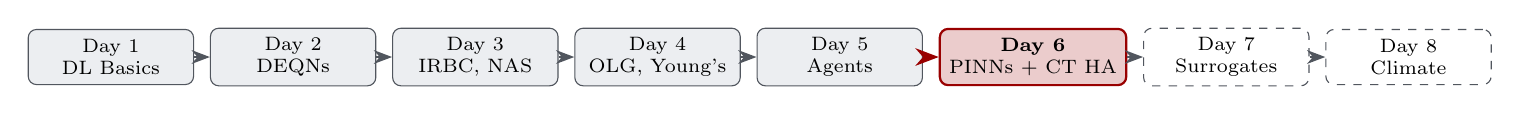
\begin{tikzpicture}[
    node distance=0.35cm and 0.2cm,
    daybox/.style={rectangle, rounded corners=3pt, minimum width=2.1cm, minimum height=0.7cm, font=\scriptsize, align=center, draw},
    done/.style={daybox, fill=uzhgreylight, draw=uzhgreydark},
    current/.style={daybox, fill=harvardcrimson!20, draw=harvardcrimson, thick},
    future/.style={daybox, fill=white, draw=uzhgreydark, dashed},
    arrow/.style={-Stealth, thick, uzhgreydark}
]
\node[done] (d1) {Day 1\\DL Basics};
\node[done, right=of d1] (d2) {Day 2\\DEQNs};
\node[done, right=of d2] (d3) {Day 3\\IRBC, NAS};
\node[done, right=of d3] (d4) {Day 4\\OLG, Young's};
\node[done, right=of d4] (d5) {Day 5\\Agents};
\node[current, right=of d5] (d6) {\textbf{Day 6}\\PINNs + CT HA};
\node[future, right=of d6] (d7) {Day 7\\Surrogates};
\node[future, right=of d7] (d8) {Day 8\\Climate};

\draw[arrow] (d1) -- (d2);
\draw[arrow] (d2) -- (d3);
\draw[arrow] (d3) -- (d4);
\draw[arrow] (d4) -- (d5);
\draw[arrow, harvardcrimson, very thick] (d5) -- (d6);
\draw[arrow, dashed] (d6) -- (d7);
\draw[arrow, dashed] (d7) -- (d8);
\end{tikzpicture}
}
\end{center}

\vspace{0.4em}
\begin{columns}[T]
\column{0.48\textwidth}
\textbf{Block 1 (PINNs):}
\begin{itemize}\itemsep2pt
    \item Single PDEs: Poisson, HJB, Black--Scholes
    \item Neural network $\approx$ PDE solution
    \item Residual loss + automatic differentiation
\end{itemize}

\column{0.48\textwidth}
\textbf{Block 2 (this block):}
\begin{itemize}\itemsep2pt
    \item \emphc{Coupled} PDEs: HJB + KFE
    \item PDEs arise from \emphc{economic equilibrium}
    \item Continuum of heterogeneous agents
\end{itemize}
\end{columns}
\end{frame}

% --- Slide 3: From PINNs to Het Agent Models ---
\begin{frame}{From PINNs to Heterogeneous Agent Models}
\begin{center}
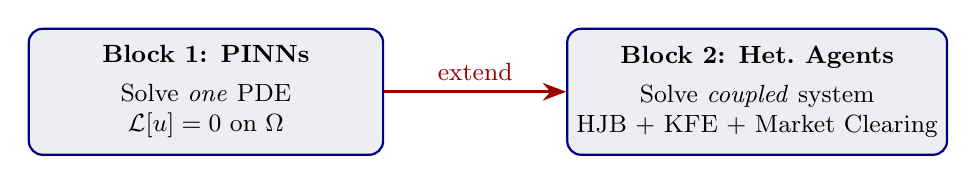
\begin{tikzpicture}[
    box/.style={rectangle, rounded corners=5pt, draw=uzhblue, thick, fill=uzhgreylight,
                 minimum width=4.5cm, minimum height=1.6cm, align=center, font=\small},
    arrow/.style={-Stealth, very thick, harvardcrimson}
]
\node[box] (pinn) at (0,0) {\textbf{Block 1: PINNs}\\[3pt]
    Solve \emph{one} PDE\\
    $\mathcal{L}[u]=0$ on $\Omega$};
\node[box] (het) at (7,0) {\textbf{Block 2: Het.\ Agents}\\[3pt]
    Solve \emph{coupled} system\\
    HJB + KFE + Market Clearing};
\draw[arrow] (pinn) -- node[above, font=\small] {extend} (het);
\end{tikzpicture}
\end{center}

\vspace{0.8em}
{\footnotesize\textbf{Recall from Deck 1:} the cake-eating HJB you just solved with a PINN is the single-PDE special case (one agent, no income, no distribution). We now \emph{add} idiosyncratic income, which forces a population density $g$ into the picture and brings the KFE alongside the HJB.}

\vspace{0.4em}
The key insight: in continuous-time macro with heterogeneous agents, \emphc{equilibrium} is characterized by a system of PDEs:
\begin{enumerate}\itemsep2pt
    \item \textbf{HJB equation} (backward): each agent optimizes $\Rightarrow$ value function $V$, policy $c^*$
    \item \textbf{Kolmogorov forward equation} (forward): population density $g$ evolves given $c^*$
    \item \textbf{Market clearing}: aggregate supply $=$ aggregate demand $\Rightarrow$ prices $r, w$
\end{enumerate}
\end{frame}

% --- Slide 4: Why Continuous Time? ---
\begin{frame}{Why Continuous Time?}
\begin{columns}[T]
\column{0.55\textwidth}
\textbf{Advantages of continuous-time formulation:}
\begin{itemize}\itemsep2pt
    \item \emphc{Analytical tractability}: Ito calculus provides closed-form FOCs
    \item \emphc{Clean separation}: HJB (backward) $\leftrightarrow$ KFE (forward)
    \item \emphc{Powerful numerical methods}: finite differences, PINNs
    \item \emphc{No expectations operator}: replaced by differential operators
    \item \emphc{Connection to mean field games} (Lasry \& Lions, 2007)
\end{itemize}

\column{0.42\textwidth}
\begin{block}{Key References}
\small
\begin{itemize}\itemsep2pt
    \item Achdou, Han, Lasry, Lions \& Moll (2022), \emph{REStud}
    \item Kaplan, Moll \& Violante (2018), \emph{AER}
    \item Moll lecture notes:\\ \url{benjaminmoll.com/lectures/}
\end{itemize}
\end{block}

\vspace{0.3em}
\begin{alertblock}{\small Discrete $\to$ Continuous}
\small
Day 4 (DEQNs, Young's method) used \emph{discrete time}.\\
Today: \emph{continuous time} $\Rightarrow$ PDEs.
\end{alertblock}
\end{columns}
\end{frame}

% --- Slide 5: Historical Context ---
\begin{frame}{The Aiyagari--Bewley--Huggett Framework}
\small
\begin{itemize}\itemsep2pt
    \item Benchmark models in ``quantitative'' macroeconomics:
    \begin{itemize}\itemsep2pt
        \item \textbf{Bewley} (1980, 1983): precautionary saving with borrowing constraints
        \item \textbf{Huggett} (1993, \emph{JEDC}): endowment economy, risk-free rate determination
        \item \textbf{Aiyagari} (1994, \emph{QJE}): production economy, general equilibrium
        \item \textbf{Krusell \& Smith} (1998, \emph{JPE}): adds aggregate TFP shocks
    \end{itemize}
    \item Core mechanism: \emphc{idiosyncratic labor income risk} is \emphc{uninsurable}
    \begin{itemize}
        \item Households want to borrow when income is low $\to$ borrowing limits prevent this
        \item Instead, households accumulate assets as \emphc{precautionary savings}
    \end{itemize}
    \item These are building blocks for \emphc{HANK} models (Kaplan, Moll \& Violante, 2018)
    \begin{itemize}
        \item Heterogeneous Agent New Keynesian: monetary/fiscal policy with inequality
    \end{itemize}
\end{itemize}
\end{frame}

% --- Slide 6: Goals ---
\begin{frame}{Goals for This Lecture}
\begin{enumerate}\itemsep3pt
    \item \textbf{Stochastic calculus refresher}: Brownian motion, Ito's lemma, Poisson processes
    \item \textbf{Derive the Kolmogorov forward equation} (KFE / Fokker--Planck):
    \begin{itemize}
        \item First as a \emphc{standalone concept from physics} (diffusion of particles)
        \item Then in \emphc{economics}: continuum of agents $\to$ wealth distribution
    \end{itemize}
    \item \textbf{The Hamilton--Jacobi--Bellman equation}: stochastic optimal control in CT
    \item \textbf{Competitive equilibrium}: coupled HJB + KFE + market clearing
    \item \textbf{The master equation}: collapsing the system into a single PDE
\end{enumerate}

\vspace{0.3em}
\begin{center}
\colorbox{uzhgreylight}{\parbox{0.8\textwidth}{\centering\small
\textbf{Deck~2} (after coffee): \emph{numerical methods} --- finite differences, PINNs, and deep learning (EMINNs) for solving these coupled PDEs.}}
\end{center}
\end{frame}

% --- Slide 7: Table of Contents ---
\begin{frame}{Table of Contents}
\tableofcontents[hideallsubsections]
\end{frame}

% --- Slide 8: References ---
\begin{frame}{Key References}
\small
\begin{columns}[T]
\column{0.48\textwidth}
\textbf{Foundational models:}
\begin{itemize}\itemsep2pt
    \item Huggett, M.\ (1993). ``The Risk-Free Rate in Heterogeneous-Agent Incomplete-Insurance Economies.'' \emph{JEDC} 17(5--6), 953--969.
    \item Aiyagari, S.R.\ (1994). ``Uninsured Idiosyncratic Risk and Aggregate Saving.'' \emph{QJE} 109(3), 659--684.
    \item Krusell, P.\ \& Smith, A.A.\ (1998). ``Income and Wealth Heterogeneity in the Macroeconomy.'' \emph{JPE} 106(5), 867--896.
\end{itemize}

\column{0.48\textwidth}
\textbf{Continuous-time formulations:}
\begin{itemize}\itemsep2pt
    \item Achdou, Han, Lasry, Lions \& Moll (2022). ``Income and Wealth Distribution in Macroeconomics: A Continuous-Time Approach.'' \emph{REStud} 89(1), 45--86.
    \item Gu, Lauriere, Merkel \& Payne (2024). ``Global Solutions to Master Equations for CT Het.\ Agent Models.'' arXiv:2406.13726.
    \item Lasry \& Lions (2007). ``Mean Field Games.'' \emph{Jpn.\ J.\ Math.}\ 2(1), 229--260.
\end{itemize}
\end{columns}
\end{frame}

% ============================================================================
% PART II: STOCHASTIC CALCULUS REFRESHER
% ============================================================================

\section{Stochastic Calculus Refresher}

\begin{frame}{}
\vfill
\begin{center}
{\Huge \textcolor{uzhblue}{\textbf{Part I}}}\\[12pt]
{\LARGE Stochastic Calculus Refresher}
\end{center}
\vfill
\end{frame}

% --- Slide: Brownian Motion Definition ---
\begin{frame}[shrink=2]{Brownian Motion (Wiener Process)}
\small
\begin{columns}[T]
\column{0.52\textwidth}
\begin{block}{Definition}
\small
A stochastic process $\{B_t\}_{t\geq 0}$ is a \emphc{standard Brownian motion} if:
\begin{enumerate}\itemsep0pt
    \item $B_0 = 0$
    \item \textbf{Independent increments}: $B_t - B_s \perp B_s - B_r$ for $r < s < t$
    \item \textbf{Gaussian}: $B_t - B_s \sim \mathcal{N}(0, t-s)$
    \item \textbf{Continuous paths}: $t \mapsto B_t$ is continuous a.s.
\end{enumerate}
\end{block}

\textbf{Key properties:}
\begin{itemize}\itemsep0pt
    \item $\E{B_t} = 0$, \; $\text{Var}(B_t) = t$
    \item Paths are \emphc{nowhere differentiable}
    \item Quadratic variation: $\langle B \rangle_t = t$
\end{itemize}

\column{0.45\textwidth}
\begin{center}
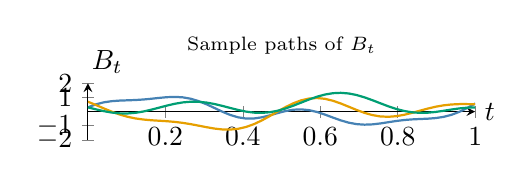
\begin{tikzpicture}
\begin{axis}[
    width=6.5cm, height=2.3cm,
    xlabel={$t$}, ylabel={$B_t$},
    xmin=0, xmax=1, ymin=-2, ymax=2,
    axis lines=middle,
    xlabel style={at={(axis description cs:1,0.5)}, anchor=west},
    ylabel style={at={(axis description cs:0.05,1)}, anchor=south},
    title={\scriptsize Sample paths of $B_t$},
    title style={at={(0.5,1.05)}},
]
% Path 1
\addplot[softblue, thick, domain=0:1, samples=50]
    {0.8*sin(deg(7*x)) + 0.5*sin(deg(13*x)) + 0.3*cos(deg(23*x))};
% Path 2
\addplot[softorange, thick, domain=0:1, samples=50]
    {-0.6*sin(deg(5*x)) + 0.7*cos(deg(11*x)) - 0.4*sin(deg(19*x))};
% Path 3
\addplot[softgreen, thick, domain=0:1, samples=50]
    {0.3*cos(deg(9*x)) - 0.5*sin(deg(17*x)) + 0.6*sin(deg(3*x))};
\end{axis}
\end{tikzpicture}
\end{center}
\end{columns}
\end{frame}

% --- Slide: Brownian Motion Intuition ---
\begin{frame}{Brownian Motion: Random Walk Limit}
\textbf{Discrete-time intuition}: Brownian motion is the limit of a scaled random walk.
\vspace{0.3em}

Let $\Delta t > 0$ and define $X_t^{\Delta t}$ by steps $\pm \sqrt{\Delta t}$ with equal probability:
\[
X_{t+\Delta t}^{\Delta t} = X_t^{\Delta t} + \sqrt{\Delta t}\;\varepsilon_t, \qquad \varepsilon_t \overset{\mathrm{iid}}{\sim} \{-1, +1\} \text{ with prob.\ } \tfrac{1}{2} \text{ each.}
\]

As $\Delta t \to 0$: \quad $X_t^{\Delta t} \;\xrightarrow{\;\mathrm{d}\;}\; B_t$ \qquad (Donsker's theorem).

\vspace{0.4em}
\begin{center}
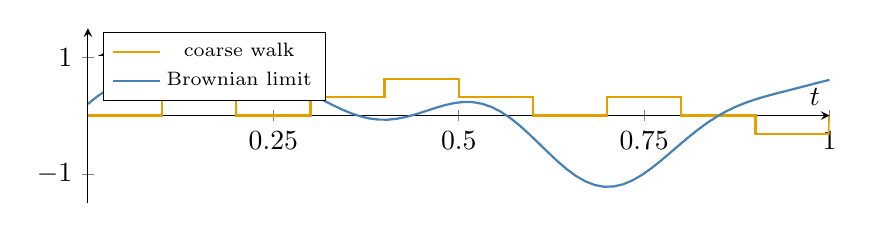
\begin{tikzpicture}
\begin{axis}[
    width=11cm, height=3.8cm,
    xlabel={$t$}, ylabel={$X_t$},
    xmin=0, xmax=1, ymin=-1.5, ymax=1.5,
    axis lines=middle,
    xtick={0,0.25,0.5,0.75,1.0},
    legend style={at={(0.02,0.98)}, anchor=north west, font=\scriptsize},
]
% Coarse random walk
\addplot[softorange, thick, const plot]
    coordinates {(0,0)(0.1,0.316)(0.2,0)(0.3,0.316)(0.4,0.632)(0.5,0.316)(0.6,0)(0.7,0.316)(0.8,0)(0.9,-0.316)(1.0,0)};
\addlegendentry{coarse walk}
% "Continuous" Brownian path
\addplot[softblue, thick, domain=0:1, samples=80]
    {0.7*sin(deg(7*x)) + 0.4*sin(deg(15*x)) + 0.2*cos(deg(23*x))};
\addlegendentry{Brownian limit}
\end{axis}
\end{tikzpicture}
\end{center}

\vspace{0.2em}
\colorbox{uzhgreylight}{\parbox{0.9\textwidth}{\centering\small
The $\sqrt{\Delta t}$ scaling is crucial: it ensures $\text{Var}(X_t) = t$, not $0$ or $\infty$.}}
\end{frame}

% --- Slide: Ito Process ---
\begin{frame}{It\^o Processes and SDEs}
\small
\begin{block}{General It\^o Process}
A stochastic process $X_t$ follows an \emphc{It\^o process} if:
\vspace{-0.3em}
\[
\boxed{dX_t = \mu(X_t, t)\ud t + \sigma(X_t, t)\ud B_t}
\]
\vspace{-0.5em}
\begin{itemize}\itemsep1pt
    \item $\mu(X_t, t)$: \emphc{drift} (deterministic trend)
    \item $\sigma(X_t, t)$: \emphc{diffusion coefficient} (volatility / noise intensity)
    \item $B_t$: standard Brownian motion
\end{itemize}
\end{block}

\vspace{0.1em}
\textbf{Important examples:}
\begin{columns}[T]
\column{0.48\textwidth}
\begin{exampleblock}{\small Geometric Brownian Motion (GBM)}
$dS_t = \mu S_t \ud t + \sigma S_t \ud B_t$\\[2pt]
{\small Used for: stock prices, GDP}
\end{exampleblock}

\column{0.48\textwidth}
\begin{exampleblock}{\small Ornstein--Uhlenbeck (OU) Process}
$dZ_t = \eta(\bar{Z} - Z_t)\ud t + \sigma \ud B_t$\\[2pt]
{\small Used for: productivity, interest rates}
\end{exampleblock}
\end{columns}
\end{frame}

% --- Slide: OU Process ---
\begin{frame}{The Ornstein--Uhlenbeck Process}
\footnotesize
\[
dZ_t = \eta(\bar{Z} - Z_t)\ud t + \sigma\ud B_t
\]

\begin{columns}[T]
\column{0.49\textwidth}
\textbf{Properties:}
\begin{itemize}\itemsep1pt
    \item \emphc{Mean-reverting}: $Z_t$ is pulled toward $\bar{Z}$ at rate $\eta$
    \item Stationary distribution: $Z_\infty \sim \mathcal{N}\!\left(\bar{Z},\; \frac{\sigma^2}{2\eta}\right)$
    \item Closed-form solution by integrating factor.
\end{itemize}

\vspace{0.1em}
\textbf{In this lecture:}
\begin{itemize}\itemsep1pt
    \item Aggregate TFP: $dZ_t = \eta(\bar{Z} - Z_t)\ud t + \sigma\ud B_t^0$
    \item Krusell--Smith (1998): $Z_t$ drives aggregate fluctuations
\end{itemize}

\column{0.47\textwidth}
\begin{center}
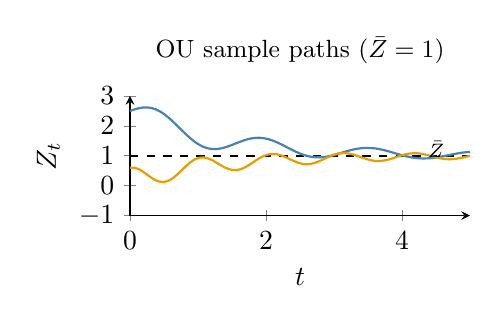
\begin{tikzpicture}
\begin{axis}[
    width=5.9cm, height=3.1cm,
    xlabel={$t$}, ylabel={$Z_t$},
    xmin=0, xmax=5, ymin=-1, ymax=3,
    axis lines=left,
    title={\small OU sample paths ($\bar{Z}=1$)},
    title style={at={(0.5,1.05)}},
]
% Mean
\addplot[dashed, black, thick, domain=0:5] {1};
% Path 1
\addplot[softblue, thick, domain=0:5, samples=80]
    {1 + 1.5*exp(-0.8*x) + 0.5*sin(deg(4*x))*exp(-0.3*x)};
% Path 2
\addplot[softorange, thick, domain=0:5, samples=80]
    {1 - 0.8*exp(-0.8*x) + 0.4*cos(deg(6*x))*exp(-0.3*x)};
\node[font=\scriptsize] at (axis cs:4.5,1.2) {$\bar{Z}$};
\end{axis}
\end{tikzpicture}
\end{center}
\end{columns}
\end{frame}

% --- Slide: Poisson Process ---
\begin{frame}{Poisson Process and Continuous-Time Markov Chains}
\small
\begin{columns}[T]
\column{0.55\textwidth}
\begin{block}{Poisson Process}
$N_t$: counting process with \emphc{intensity} $\lambda > 0$.
\begin{itemize}\itemsep1pt
    \item Jumps of size $+1$ at random times
    \item Inter-arrival times $\sim \text{Exp}(\lambda)$
    \item $\Pr(\text{jump in } [t, t+h)) = \lambda h + o(h)$
\end{itemize}
\end{block}

\vspace{0.2em}
\textbf{Income switching} (for our models):
\begin{itemize}\itemsep2pt
    \item Labor state $n_t \in \{n_1, n_2\}$ (e.g., employed/unemployed)
    \item $n_1 \to n_2$ with intensity $\lambda_1$
    \item $n_2 \to n_1$ with intensity $\lambda_2$
    \item Ergodic probabilities: $\pi_1 = \frac{\lambda_2}{\lambda_1+\lambda_2}$, $\pi_2 = \frac{\lambda_1}{\lambda_1+\lambda_2}$
\end{itemize}

\column{0.42\textwidth}
\begin{center}
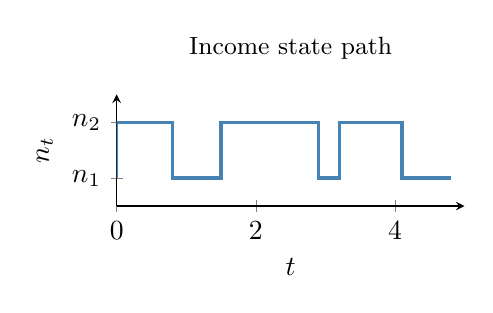
\begin{tikzpicture}
% Poisson jump path
\begin{axis}[
    width=6cm, height=3cm,
    xlabel={$t$}, ylabel={$n_t$},
    xmin=0, xmax=5, ymin=0.5, ymax=2.5,
    axis lines=left,
    ytick={1,2}, yticklabels={$n_1$, $n_2$},
    title={\small Income state path},
    title style={at={(0.5,1.08)}, font=\small},
]
\addplot[softblue, very thick, const plot mark right]
    coordinates {(0,1)(0.8,2)(1.5,1)(2.9,2)(3.2,1)(4.1,2)(4.8,1)};
\end{axis}
\end{tikzpicture}

\vspace{0.2em}
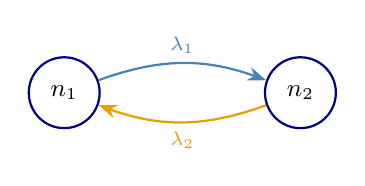
\begin{tikzpicture}[
    state/.style={circle, draw=uzhblue, thick, minimum size=0.9cm, font=\small},
    arrow/.style={-Stealth, thick}
]
\node[state] (n1) at (0,0) {$n_1$};
\node[state] (n2) at (3,0) {$n_2$};
\draw[arrow, softblue, bend left=20] (n1) to node[above, font=\scriptsize] {$\lambda_1$} (n2);
\draw[arrow, softorange, bend left=20] (n2) to node[below, font=\scriptsize] {$\lambda_2$} (n1);
\end{tikzpicture}
\end{center}
\end{columns}
\end{frame}

% --- Slide: Ito's Lemma ---
\begin{frame}{It\^o's Lemma: The Chain Rule of Stochastic Calculus}
\begin{block}{It\^o's Lemma}
Let $X_t$ follow $dX_t = \mu\ud t + \sigma\ud B_t$ and let $f \in C^2$. Then:
\[
\boxed{df(X_t) = \left[f'(X_t)\,\mu + \tfrac{1}{2}f''(X_t)\,\sigma^2\right]\ud t + f'(X_t)\,\sigma\,\ud B_t}
\]
\end{block}

\vspace{0.2em}
\textbf{The key difference from ordinary calculus:}
\begin{itemize}\itemsep2pt
    \item In ordinary calculus: $df = f'\,dX$ \quad (first-order only)
    \item In stochastic calculus: $df = f'\,dX + \frac{1}{2}f''\,(dX)^2$ \quad (second-order term survives!)
    \item Why? Because $(dB_t)^2 = dt \neq 0$ (Brownian motion has ``infinite'' variation)
\end{itemize}

\vspace{0.3em}
\begin{center}
\colorbox{uzhgreylight}{\parbox{0.7\textwidth}{\centering
\textbf{Differential algebra rules:}\\[4pt]
$\ud t \cdot \ud t = 0$, \qquad $\ud t \cdot \ud B_t = 0$, \qquad $\emphc{\ud B_t \cdot \ud B_t = \ud t}$
}}
\end{center}
\end{frame}

% --- Slide: Ito's Lemma Example ---
\begin{frame}{It\^o's Lemma: Worked Example}
\textbf{Example}: Let $dX_t = \mu X_t\ud t + \sigma X_t\ud B_t$ (GBM). Find $d(\ln X_t)$.

\vspace{0.3em}
\textbf{Step 1}: Let $f(x) = \ln x$, so $f'(x) = 1/x$, $f''(x) = -1/x^2$.

\vspace{0.2em}
\textbf{Step 2}: Apply It\^o's Lemma with $\mu(X_t) = \mu X_t$, $\sigma(X_t) = \sigma X_t$:
\begin{align*}
d(\ln X_t) &= \frac{1}{X_t}\cdot \mu X_t\ud t + \frac{1}{2}\left(-\frac{1}{X_t^2}\right)(\sigma X_t)^2\ud t + \frac{1}{X_t}\cdot \sigma X_t \ud B_t \\[6pt]
&= \boxed{\left(\mu - \tfrac{1}{2}\sigma^2\right)\ud t + \sigma\ud B_t}
\end{align*}

\vspace{0.2em}
\textbf{Insight}: $\ln X_t$ is an It\^o process with \emph{constant} drift $\mu - \frac{1}{2}\sigma^2$ and diffusion $\sigma$.

\vspace{0.2em}
$\Rightarrow$ Solution: $X_t = X_0 \exp\!\left[\left(\mu - \tfrac{1}{2}\sigma^2\right)t + \sigma B_t\right]$

\vspace{0.2em}
{\small The $-\frac{1}{2}\sigma^2$ \emphc{It\^o correction} is why expected return $\neq$ log return for volatile assets.}
\end{frame}

% --- Slide: Multivariate Ito ---
\begin{frame}{It\^o's Lemma: Multivariate Version}
\small
For $V(X_t, t)$ where $dX_t = \mu\ud t + \sigma\ud B_t$:
\[
\boxed{dV = \left[\frac{\partial V}{\partial t} + \mu\frac{\partial V}{\partial x} + \frac{1}{2}\sigma^2 \frac{\partial^2 V}{\partial x^2}\right]\ud t + \sigma\frac{\partial V}{\partial x}\,\ud B_t}
\]

\vspace{0.2em}
\textbf{With jumps} (Poisson process with intensity $\lambda$, jump $\Delta X$):
\[
dV = \underbrace{\left[\frac{\partial V}{\partial t} + \mu\frac{\partial V}{\partial x} + \frac{1}{2}\sigma^2 \frac{\partial^2 V}{\partial x^2}\right]\ud t + \sigma\frac{\partial V}{\partial x}\ud B_t}_{\text{diffusion part}} + \underbrace{\left[V(X_{t^-}+\Delta X, t) - V(X_{t^-}, t)\right]\ud N_t}_{\text{jump part}}
\]

\vspace{0.2em}
\begin{center}
\colorbox{uzhgreylight}{\parbox{0.8\textwidth}{\centering\small
We will use the multivariate version repeatedly:\\
\textbf{HJB derivation} (Part~IV) and \textbf{KFE derivation} (Part~II).}}
\end{center}
\end{frame}

% ============================================================================
% PART III: THE KOLMOGOROV FORWARD EQUATION
% ============================================================================

\section{The Kolmogorov Forward Equation}

\begin{frame}{}
\vfill
\begin{center}
{\Huge \textcolor{uzhblue}{\textbf{Part II}}}\\[12pt]
{\LARGE The Kolmogorov Forward Equation}\\[6pt]
{\large (Fokker--Planck Equation)}
\end{center}
\vfill
\end{frame}

% --- Slide: What is the KFE ---
\begin{frame}{What Is the Kolmogorov Forward Equation?}
\small
\begin{columns}[T]
\column{0.58\textwidth}
The \emphc{Kolmogorov forward equation} (KFE), also known as the \emphc{Fokker--Planck equation}, describes how the \textbf{probability density} of a stochastic process evolves over time.

\vspace{0.3em}
\textbf{Origin}: physics and applied mathematics.
\begin{itemize}\itemsep2pt
    \item \textbf{A.N.\ Kolmogorov} (1931): general theory of continuous Markov processes
    \item \textbf{A.D.\ Fokker} (1914) \& \textbf{M.\ Planck} (1917): diffusion of particles
    \item Applications: heat conduction, fluid dynamics, plasma physics, chemical kinetics, population genetics, neuroscience, \ldots
\end{itemize}

\column{0.38\textwidth}
\begin{center}

\includegraphics[width=0.78\linewidth,height=0.34\textheight,keepaspectratio]{images/kolmogorov.jpg}\\[-2pt]
{\tiny A.N.\ Kolmogorov, Wikimedia Commons}
\end{center}
\end{columns}

\vspace{0.1em}
{\small \textbf{Key idea}: micro dynamics (drift + noise) $\Rightarrow$ macro density law of motion.}
\end{frame}

% --- Slide: Standalone KFE - Pure Diffusion ---
\begin{frame}{Standalone Example: Diffusion of Particles}
\small
\textbf{Setup (no economics!)}: Consider a large population of particles, each independently following:
\[
dX_t = \mu\ud t + \sigma\ud B_t
\]
where $\mu$ is a constant drift and $\sigma$ is a constant diffusion coefficient.

\vspace{0.2em}
\textbf{Question}: If at time $t=0$ the particles have density $g_0(x)$, what is the density $g(x,t)$ at time $t > 0$?

\vspace{0.2em}
\begin{block}{Kolmogorov Forward Equation (constant coefficients)}
\vspace{-0.3em}
\[
\boxed{\frac{\partial g}{\partial t}(x,t) = -\mu\frac{\partial g}{\partial x}(x,t) + \frac{\sigma^2}{2}\frac{\partial^2 g}{\partial x^2}(x,t)}
\]
\vspace{-0.3em}
\end{block}

\vspace{0.2em}
\textbf{Two competing effects:}
\begin{itemize}\itemsep2pt
    \item $-\mu\,\partial_x g$: \emphc{advection} --- drift transports the density
    \item $\frac{\sigma^2}{2}\partial_{xx}g$: \emphc{diffusion} --- noise spreads the density
\end{itemize}
\end{frame}

% --- Slide: KFE Derivation from First Principles ---
\begin{frame}{Deriving the KFE from First Principles}
\small
\textbf{Goal}: Derive $\partial_t g = -\mu\partial_x g + \frac{\sigma^2}{2}\partial_{xx} g$ from basic probability.

\vspace{0.1em}
\textbf{Step 1} --- For any smooth test function $\varphi(x)$:
$\E{\varphi(X_t)} = \int_{-\infty}^{\infty} \varphi(x)\,g(x,t)\ud x$

\textbf{Step 2} --- Differentiate w.r.t.\ $t$ and use It\^o's lemma on $\varphi(X_t)$:
\[
\frac{d}{dt}\int \varphi\, g\ud x = \E{\mu\,\varphi'(X_t) + \tfrac{\sigma^2}{2}\varphi''(X_t)} = \int \left[\mu\,\varphi' + \tfrac{\sigma^2}{2}\varphi''\right] g\ud x
\]

\vspace{-0.3em}
\textbf{Step 3} --- Integrate by parts (assuming $g \to 0$ at $\pm\infty$):
\vspace{-0.3em}
\begin{align*}
\int \mu\,\varphi'\, g \ud x &= -\int \varphi\,\mu\,\partial_x g\ud x & \text{(once)}\\
\int \tfrac{\sigma^2}{2}\varphi''\, g\ud x &= \int \varphi\,\tfrac{\sigma^2}{2}\partial_{xx}g\ud x & \text{(twice)}
\end{align*}

\vspace{-0.3em}
\textbf{Step 4} --- Since this holds for \emph{all} test functions $\varphi$:
$\boxed{\partial_t g = -\mu\,\partial_x g + \tfrac{\sigma^2}{2}\,\partial_{xx} g} \quad \checkmark$
\end{frame}

% --- Slide: KFE General Form ---
\begin{frame}{The KFE: General It\^o Diffusion}
\small
For $dX_t = \mu(X_t)\ud t + \sigma(X_t)\ud B_t$ with \emphc{state-dependent} drift and diffusion,
the density $g(x,t)$ satisfies the \textbf{general KFE}:

\begin{block}{Kolmogorov Forward / Fokker--Planck Equation}
\vspace{-0.5em}
\[
\boxed{\frac{\partial g}{\partial t}(x,t) = -\frac{\partial}{\partial x}\big[\mu(x)\,g(x,t)\big] + \frac{1}{2}\frac{\partial^2}{\partial x^2}\big[\sigma(x)^2\,g(x,t)\big]}
\]
\vspace{-0.5em}
\end{block}

\textbf{Important}: when $\sigma$ depends on $x$, it enters \emph{inside} the second derivative:
$\frac{1}{2}\partial_{xx}\!\left[\sigma(x)^2 g\right] \;\neq\; \frac{\sigma(x)^2}{2}\partial_{xx}g$

In \emphc{divergence form}: $\partial_t g = -\partial_x\underbrace{\left[\mu(x)g - \frac{1}{2}\partial_x(\sigma^2 g)\right]}_{=:\text{probability flux } J(x,t)}$
\quad Conservation law: $\partial_t g + \partial_x J = 0$.
\end{frame}

% --- Slide: Example - Heat Equation ---
\begin{frame}{Example 1: The Heat Equation (Pure Diffusion)}
\small
\textbf{Setting}: No drift ($\mu = 0$), constant diffusion $\sigma$. Particles start at $x_0$:
$\partial_t g = \frac{\sigma^2}{2}\partial_{xx}g$, \; $g(x,0) = \delta(x - x_0)$.

\textbf{Solution}: Gaussian with spreading variance:
$g(x,t) = \frac{1}{\sqrt{2\pi\sigma^2 t}}\exp\!\left(-\frac{(x-x_0)^2}{2\sigma^2 t}\right)$

\begin{columns}[T]
\column{0.55\textwidth}
\begin{center}
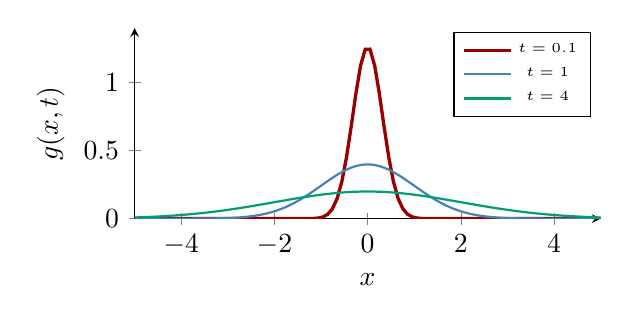
\begin{tikzpicture}
\begin{axis}[
    width=7.5cm, height=4cm,
    xlabel={$x$}, ylabel={$g(x,t)$},
    xmin=-5, xmax=5, ymin=0, ymax=1.4,
    ytick={0,0.5,1.0},
    axis lines=left,
    legend style={at={(0.98,0.98)}, anchor=north east, font=\tiny},
]
\addplot[harvardcrimson, very thick, domain=-5:5, samples=100]
    {exp(-x^2/0.2) / sqrt(0.2*3.14159)};
\addlegendentry{$t=0.1$}
\addplot[softblue, thick, domain=-5:5, samples=100]
    {exp(-x^2/2) / sqrt(2*3.14159)};
\addlegendentry{$t=1$}
\addplot[softgreen, thick, domain=-5:5, samples=100]
    {exp(-x^2/8) / sqrt(8*3.14159)};
\addlegendentry{$t=4$}
\end{axis}
\end{tikzpicture}
\end{center}

\column{0.42\textwidth}
\textbf{Physical interpretation:}
\begin{itemize}\itemsep1pt
    \item Heat spreads from a point source
    \item Variance grows linearly: $\text{Var} = \sigma^2 t$
    \item Total ``mass'' conserved: $\int g = 1$
    \item \emphc{Most fundamental PDE in physics}
\end{itemize}

\vspace{0.2em}
{\small This is exactly what PINNs solve (Day~5)!}
\end{columns}
\end{frame}

% --- Slide: Example - OU Process KFE ---
\begin{frame}{Example 2: Ornstein--Uhlenbeck Process}
\small
\textbf{Setting}: $dX_t = \theta(\bar{x} - X_t)\ud t + \sigma\ud B_t$ \quad (mean-reverting).

\vspace{0.2em}
\textbf{KFE}: $\partial_t g = \theta\,\partial_x\!\left[(x - \bar{x})\,g\right] + \frac{\sigma^2}{2}\partial_{xx}g$

\vspace{0.2em}
\textbf{Stationary distribution} ($\partial_t g = 0$):
\[
\boxed{g^*(x) = \frac{1}{\sqrt{2\pi\sigma^2/(2\theta)}}\exp\!\left(-\frac{(x-\bar{x})^2}{2\cdot\sigma^2/(2\theta)}\right) = \mathcal{N}\!\left(\bar{x},\;\frac{\sigma^2}{2\theta}\right)}
\]

\begin{columns}[T]
\column{0.55\textwidth}
\begin{center}
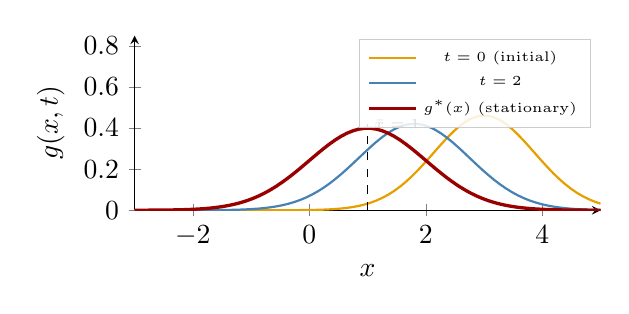
\begin{tikzpicture}
\begin{axis}[
    width=7.5cm, height=3.8cm,
    xlabel={$x$}, ylabel={$g(x,t)$},
    xmin=-3, xmax=5, ymin=0, ymax=0.85,
    axis lines=left,
    legend style={at={(0.98,0.98)}, anchor=north east, font=\tiny,
                  fill=white, fill opacity=0.85, draw=gray!40, text opacity=1},
]
% Initial (spread)
\addplot[softorange, thick, domain=-3:5, samples=80]
    {exp(-(x-3)^2/1.5) / sqrt(1.5*3.14159)};
\addlegendentry{$t=0$ (initial)}
% Intermediate
\addplot[softblue, thick, domain=-3:5, samples=80]
    {exp(-(x-1.8)^2/1.8) / sqrt(1.8*3.14159)};
\addlegendentry{$t=2$}
% Stationary
\addplot[harvardcrimson, very thick, domain=-3:5, samples=80]
    {exp(-(x-1)^2/2) / sqrt(2*3.14159)};
\addlegendentry{$g^*(x)$ (stationary)}
\draw[dashed] (axis cs:1,0) -- (axis cs:1,0.42);
\node[font=\tiny] at (axis cs:1.5,0.42) {$\bar{x}=1$};
\end{axis}
\end{tikzpicture}
\end{center}

\column{0.42\textwidth}
\textbf{Interpretation:}
\begin{itemize}\itemsep2pt
    \item Mean reversion ($\theta$) concentrates mass around $\bar{x}$
    \item Diffusion ($\sigma$) spreads mass
    \item Balance $\Rightarrow$ Gaussian steady state
    \item Larger $\theta$ $\Rightarrow$ tighter distribution
\end{itemize}

\vspace{0.2em}
{\small This will model \emphc{aggregate productivity} $Z_t$ in the Krusell--Smith model.}
\end{columns}
\end{frame}

% --- Slide: Example - Drift-Diffusion with Absorbing BC ---
\begin{frame}{Example 3: Boundaries and Borrowing Constraints}
\small
\textbf{Setting}: $dX_t=\mu\ud t+\sigma\ud B_t$ on $X_t\ge 0$.

\begin{columns}[T]
\column{0.56\textwidth}
\begin{itemize}\itemsep2pt
    \item \textbf{Absorbing BC}: mass exits at the boundary.
    \item \textbf{Reflecting BC}: no net probability flow across the boundary.
    \item In Huggett/Aiyagari (asset drift only), borrowing constraint $a\ge\ubar a$ is a \emphc{state constraint}.
\end{itemize}

\vspace{0.1em}
For the absolutely continuous density part:
\[
J(a,n):=s(a,n)\,g_t(a,n),\qquad J(\ubar a,n)=0.
\]
Boundary atoms can form at $\ubar a$ when constrained agents pile up.

\column{0.40\textwidth}
\begin{center}
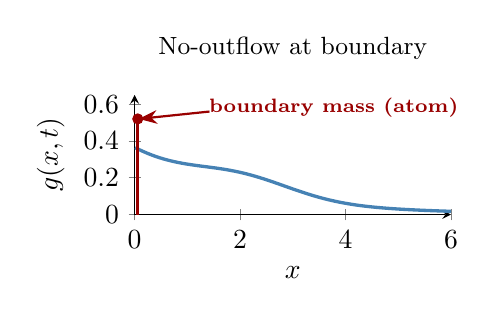
\begin{tikzpicture}
\begin{axis}[
    width=5.6cm, height=3.1cm,
    xlabel={$x$}, ylabel={$g(x,t)$},
    xmin=0, xmax=6, ymin=0, ymax=0.65,
    axis lines=left,
    clip=false,
    title={\small No-outflow at boundary},
    title style={at={(0.5,1.08)}, font=\small},
]
\addplot[softblue, very thick, domain=0.01:6, samples=80]
    {0.35*exp(-0.5*(x-0.01)) + 0.1*exp(-(x-2)^2/2)};
\draw[harvardcrimson, very thick] (axis cs:0.06,0) -- (axis cs:0.06,0.52);
\addplot[harvardcrimson, only marks, mark=*, mark size=1.8pt]
    coordinates {(0.06,0.52)};
\node[font=\scriptsize\bfseries, harvardcrimson, fill=white, inner sep=1pt, anchor=west]
    at (axis cs:1.35,0.58) {boundary mass (atom)};
\draw[harvardcrimson, thick, -Stealth] (axis cs:1.42,0.56) -- (axis cs:0.08,0.52);
\end{axis}
\end{tikzpicture}
\end{center}
\end{columns}
\end{frame}

% --- Slide: From Physics to Economics ---
\begin{frame}{From Physics to Economics: A Continuum of Agents}
\small
\textbf{Key insight} (propagation of chaos):

\vspace{0.1em}
Consider a \emphc{continuum} of agents $i \in [0,1]$, each independently following:
\[
dX_t^i = \mu(X_t^i)\ud t + \sigma(X_t^i)\ud B_t^i
\]
where $B_t^i$ are \emph{independent} Brownian motions (idiosyncratic shocks).

\vspace{0.2em}
By the \textbf{law of large numbers} at the population level:
\begin{itemize}\itemsep2pt
    \item The \emphc{cross-sectional density} $g(x,t)$ evolves \emphc{deterministically}
    \item Even though each individual path is random!
    \item The density satisfies the \emphc{KFE}: $\partial_t g = -\partial_x[\mu g] + \frac{1}{2}\partial_{xx}[\sigma^2 g]$
\end{itemize}

\vspace{0.2em}
\begin{center}
\colorbox{uzhgreylight}{\parbox{0.85\textwidth}{\centering
\textbf{Analogy}: Each molecule of air moves randomly (Brownian motion),\\
but the \emph{temperature distribution} in a room evolves deterministically (heat equation).\\[3pt]
In economics: each household's income is random,\\
but the \emph{wealth distribution} evolves deterministically (KFE).
}}
\end{center}
\end{frame}

% --- Slide: KFE in Economics ---
\begin{frame}{KFE in Economics: The Wealth Distribution}
\small
\textbf{Setup}: Agent $i$ has wealth $a_t^i$ and income state $n_t^i \in \{n_1, n_2\}$.

\vspace{0.1em}
Individual wealth evolves as:
\[
da_t^i = \underbrace{s(a_t^i, n_t^i)}_{\text{savings = income} - \text{consumption}}\ud t, \qquad a_t^i \geq \ubar{a}
\]
Income $n_t^i$ switches between $n_1 \leftrightarrow n_2$ with Poisson intensities $\lambda_1, \lambda_2$.

\vspace{0.1em}
The \emphc{cross-sectional density} $g_t(a, n)$ satisfies:
\[
\boxed{\partial_t g_t(a,n) = -\partial_a\!\left[s(a,n)\,g_t(a,n)\right] - \lambda(n)\,g_t(a,n) + \lambda(\hat{n})\,g_t(a,\hat{n})}
\]
where $\hat{n}$ denotes the complementary income state.

\vspace{0.1em}
\begin{itemize}\itemsep2pt
    \item $-\partial_a[s \cdot g]$: flow of agents along the wealth axis (savings)
    \item $-\lambda(n)\,g(a,n)$: agents \emphc{leaving} state $n$ \quad {\small (exit from $n \to \hat{n}$)}
    \item $+\lambda(\hat{n})\,g(a,\hat{n})$: agents \emphc{entering} state $n$ \quad {\small (entry from $\hat{n} \to n$)}
\end{itemize}
\end{frame}

% --- Slide: KFE Stationary ---
\begin{frame}{Stationary Wealth Distribution}
Setting $\partial_t g = 0$, the \emphc{stationary} (ergodic) distribution solves:
\[
\begin{aligned}
0 ={}& -\partial_a\!\left[s(a,n)\,g^*(a,n)\right] \\
& - \lambda(n)\,g^*(a,n) + \lambda(\hat{n})\,g^*(a,\hat{n})
\end{aligned}
\]

\begin{columns}[T]
\column{0.50\textwidth}
\textbf{Key features of $g^*(a,n)$:}
\begin{itemize}\itemsep2pt
    \item \emphc{Right-skewed}: many poor, few rich
    \item \emphc{Mass point} at borrowing constraint $\ubar{a}$ for low-income agents
    \item Separate densities for each income state
    \item Normalization: $\sum_n \int_{\ubar{a}}^{\infty} g^*(a,n)\ud a = 1$
\end{itemize}

\vspace{0.2em}
{\small This is the object solved numerically in Aiyagari (1994) and Achdou et al.\ (2022).}

\column{0.46\textwidth}
\begin{center}
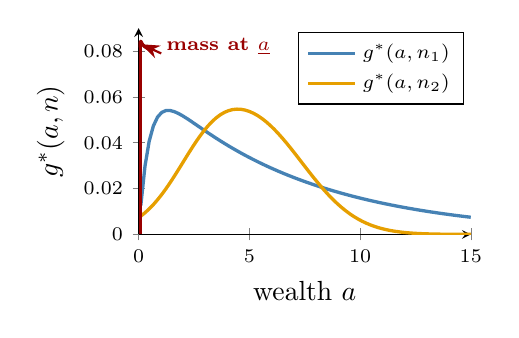
\begin{tikzpicture}
\begin{axis}[
    width=5.8cm, height=4.2cm,
    xlabel={wealth $a$}, ylabel={$g^*(a,n)$},
    xmin=0, xmax=15, ymin=0, ymax=0.09,
    axis lines=left,
    scaled y ticks=false,
    ytick={0,0.02,0.04,0.06,0.08},
    yticklabels={0,0.02,0.04,0.06,0.08},
    tick label style={font=\scriptsize},
    label style={font=\normalsize},
    legend style={at={(0.98,0.98)}, anchor=north east, font=\scriptsize},
]
% Low income state - peaked at low wealth
\addplot[softblue, very thick, domain=0.1:15, samples=80]
    {0.07*exp(-0.15*(x-0.1)) * (1 - exp(-2*x))};
\addlegendentry{$g^*(a, n_1)$}
% High income state - spread to higher wealth
\addplot[softorange, very thick, domain=0.1:15, samples=80]
    {0.05*exp(-(x-5)^2/12) + 0.01*exp(-(x-3)^2/4)};
\addlegendentry{$g^*(a, n_2)$}
% Mass point arrow at borrowing constraint
\draw[harvardcrimson, very thick, ->] (axis cs:0.1,0) -- (axis cs:0.1,0.085);
\node[font=\scriptsize\bfseries, harvardcrimson, fill=white, inner sep=1pt, anchor=west]
    at (axis cs:1.1,0.082) {mass at $\ubar{a}$};
\draw[harvardcrimson, thick, -Stealth] (axis cs:1.02,0.079) -- (axis cs:0.12,0.083);
\end{axis}
\end{tikzpicture}
\end{center}
\end{columns}
\end{frame}

% --- Slide: KFE Why No Aggregate Brownian ---
\begin{frame}{Why Does the KFE Not Have a $dB_t^0$ Term?}
\small
\textbf{Observation}: The KFE for $g_t(a,n)$ is a \emphc{deterministic} PDE, even though each agent faces random shocks.

\vspace{0.1em}
\textbf{Why?}
\begin{itemize}\itemsep0pt
    \item Agents face \emphc{idiosyncratic} shocks $dB_t^i$ (independent across $i$)
    \item By the \textbf{law of large numbers}: randomness washes out at the population level
    \item $\Rightarrow$ The density $g_t$ evolves \emphc{deterministically}
\end{itemize}

\vspace{0.1em}
\textbf{When would $dB_t^0$ appear in the KFE?}
\begin{itemize}\itemsep0pt
    \item If there are \emphc{aggregate shocks} (e.g., TFP $Z_t$ following an OU process)
    \item Then prices $r_t, w_t$ become stochastic $\Rightarrow$ drift is stochastic
    \item $\Rightarrow$ The density $g_t$ becomes a \emphc{stochastic process} adapted to $\mathcal{F}_t^0$
    \item This is the \emphc{Krusell--Smith} (1998) setting --- much harder!
\end{itemize}

\vspace{0.1em}
{\centering\scriptsize
\textbf{Aiyagari} (no aggregate shocks): KFE is deterministic $\checkmark$ \quad
\textbf{Krusell--Smith} (aggregate shocks): KFE is stochastic $\Rightarrow$ ``master equation''\\}
\end{frame}

% --- Slide: KFE and Mean Field Games ---
\begin{frame}{Connection to Mean Field Games}
\small
The KFE is one half of the \emphc{Mean Field Game} (MFG) system:

\begin{center}
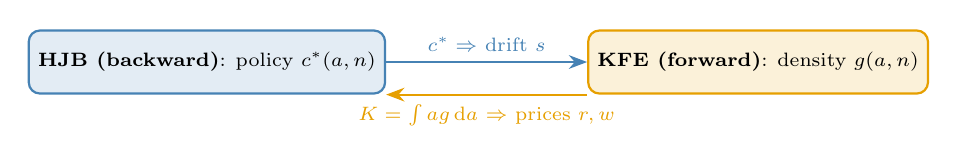
\begin{tikzpicture}[
    box/.style={rectangle, rounded corners=4pt, draw, thick, minimum width=3.8cm, minimum height=0.8cm, align=center, font=\scriptsize},
    arrow/.style={-Stealth, thick}
]
\node[box, fill=softblue!15, draw=softblue] (hjb) at (0,0.6) {\textbf{HJB (backward)}: policy $c^*(a,n)$};
\node[box, fill=softorange!15, draw=softorange] (kfe) at (7,0.6) {\textbf{KFE (forward)}: density $g(a,n)$};

\draw[arrow, softblue] (hjb.east) -- node[above, font=\scriptsize] {$c^* \Rightarrow$ drift $s$} (kfe.west);
\draw[arrow, softorange] (kfe.south west) -- node[below, font=\scriptsize] {$K = \int ag\ud a$ $\Rightarrow$ prices $r, w$} (hjb.south east);
\end{tikzpicture}
\end{center}

\vspace{-0.2em}
\begin{itemize}\itemsep0pt
    \item \textbf{Lasry \& Lions} (2007): formalized MFGs as coupled PDE systems
    \item In economics: ``Mean Field Game'' $=$ \emphc{competitive equilibrium} with continuum of agents
    \item Each agent is ``small'' $\Rightarrow$ takes distribution as given
    \item But collectively, agents \emph{determine} the distribution
    \item \emphc{Fixed point}: beliefs about $g$ are consistent with optimal behavior
\end{itemize}
\end{frame}

% --- Slide: KFE Summary ---
\begin{frame}{KFE: Summary}
\small
\begin{center}
\renewcommand{\arraystretch}{1.2}
\begin{tabular}{lll}
\toprule
\textbf{Version} & \textbf{KFE} & \textbf{Application} \\
\midrule
Pure diffusion & $\partial_t g = -\mu\partial_x g + \frac{\sigma^2}{2}\partial_{xx}g$ & Heat equation, particle diffusion \\[4pt]
General It\^o & $\partial_t g = -\partial_x[\mu g] + \frac{1}{2}\partial_{xx}[\sigma^2 g]$ & OU process, GBM \\[4pt]
With Poisson & $\cdots - \lambda(n)g(n) + \lambda(\hat{n})g(\hat{n})$ & Income switching \\[4pt]
Economic & drift $= s(a,n)$ (endogenous) & Wealth distribution \\
\bottomrule
\end{tabular}
\end{center}

\vspace{0.2em}
\textbf{Key takeaways:}
\begin{itemize}\itemsep2pt
    \item The KFE maps $\{\text{drift } \mu, \text{diffusion } \sigma, \text{initial density } g_0\} \to$ density evolution $g(x,t)$
    \item In economics: drift $=$ savings (\emphc{endogenous}, from HJB)
    \item Without aggregate shocks: KFE is \emphc{deterministic} (LLN)
    \item With aggregate shocks: KFE becomes \emphc{stochastic} $\Rightarrow$ ``master equation''
    \item State constraints can require boundary atoms in addition to an interior density
\end{itemize}
\end{frame}

% ============================================================================
% PART IV: THE HJB EQUATION
% ============================================================================

\section{The HJB Equation}

\begin{frame}{}
\vfill
\begin{center}
{\Huge \textcolor{uzhblue}{\textbf{Part III}}}\\[12pt]
{\LARGE The Hamilton--Jacobi--Bellman Equation}\\[6pt]
{\large Stochastic Optimal Control in Continuous Time}
\end{center}
\vfill
\end{frame}

% --- Slide: The Agent's Problem ---
\begin{frame}{The Agent's Optimization Problem}
\textbf{Setup}: Agent $i$ with state $x_t^i = (a_t^i, n_t^i)$ chooses consumption $c_t^i$ to solve:
\[
\max_{\{c_t^i\}_{t\geq 0}} \;\E{\int_0^\infty e^{-\rho t}\,u(c_t^i)\ud t}
\]
subject to:
\begin{align*}
da_t^i &= \underbrace{(\tilde{w}_t n_t^i + \tilde{r}_t a_t^i - c_t^i)}_{\equiv\; s(c_t^i,\, a_t^i,\, n_t^i,\, \tilde{w}_t,\, \tilde{r}_t)}\ud t, \qquad a_t^i \geq \ubar{a} \\[4pt]
n_t^i &\in \{n_1, n_2\}, \quad \text{switches with Poisson intensity } \lambda(n_t^i)
\end{align*}

\vspace{0.2em}
\begin{itemize}\itemsep2pt
    \item $u(c) = \frac{c^{1-\gamma}}{1-\gamma}$: CRRA utility, $\gamma > 0$ (risk aversion)
    \item $\rho > 0$: discount rate
    \item $(\tilde{r}, \tilde{w})$: agent's \emphc{beliefs} about price processes (rental rate, wage)
    \item $\ubar{a}$: exogenous borrowing limit
\end{itemize}
\end{frame}

% --- Slide: Value Function ---
\begin{frame}{The Value Function}
\small
\begin{block}{Definition}
The \emphc{value function} $V(a, n)$ is the maximum expected discounted utility starting from state $(a,n)$:
\[
V(a, n) = \max_{\{c_t\}} \;\E{\int_0^\infty e^{-\rho t}\,u(c_t)\ud t \;\Big|\; a_0 = a,\; n_0 = n}
\]
\end{block}

\vspace{0.3em}
\textbf{Properties of $V$:}
\begin{itemize}\itemsep2pt
    \item $V$ is \emphc{increasing} in $a$ (more wealth $\Rightarrow$ higher utility)
    \item $V$ is \emphc{concave} in $a$ (diminishing marginal value of wealth)
    \item $V(a, n_2) > V(a, n_1)$ if $n_2 > n_1$ (higher income $\Rightarrow$ higher value)
    \item $V'(a) = \partial_a V(a,n)$ is the \emphc{marginal value of wealth}
\end{itemize}

\vspace{0.2em}
\textbf{Goal}: Find $V(a,n)$ and the optimal policy $c^*(a,n)$.
$\Rightarrow$ Use the \emphc{Hamilton--Jacobi--Bellman equation}.
\end{frame}

% --- Slide: HJB Derivation Step by Step ---
\begin{frame}{Deriving the HJB: Five Steps}
\small
\textbf{Step 1} --- \emphc{Dynamic Programming Principle}. For small $h > 0$:
\[
V(a,n) = \max_c \left\{\int_0^h e^{-\rho t}u(c_t)\ud t + e^{-\rho h}\,\E{V(a_h, n_h) \mid a_0=a, n_0=n}\right\}
\]

\textbf{Step 2} --- \emphc{It\^o's lemma} on $V(a_t, n_t)$ (between jumps of $n$):
\[
dV = V'(a,n)\cdot s(c,a,n)\ud t
\]
(no diffusion term since $da = s\ud t$ is deterministic between jumps)

\textbf{Step 3} --- \emphc{Take expectations}, account for Poisson jumps:
\[
\E{dV} = \left[V'(a,n)\cdot s + \lambda(n)\big(V(a,\hat{n}) - V(a,n)\big)\right]\ud t
\]

\textbf{Step 4} --- \emphc{Substitute} into DPP, divide by $h$, let $h \to 0$:

\textbf{Step 5} --- \emphc{Impose optimality} over $c$:
\[
\boxed{\rho V(a,n) = \max_c\left\{u(c) + V'(a,n)\cdot(wn + ra - c) + \lambda(n)\big(V(a,\hat{n}) - V(a,n)\big)\right\}}
\]
\end{frame}

% --- Slide: HJB Interpretation ---
\begin{frame}{The HJB Equation: Interpretation}
\[
\rho V(a,n) = \max_c\Big\{u(c) + \underbrace{V'(a,n)\cdot s(a,n,c)}_{\text{marginal value $\times$ savings}} + \underbrace{\lambda(n)\big(V(a,\hat{n}) - V(a,n)\big)}_{\text{expected change from income switch}}\Big\}
\]

\vspace{0.2em}
\textbf{Interpretation} (``required return on the value function''):
\begin{itemize}\itemsep2pt
    \item \emphc{LHS}: $\rho V$ = ``required return'' = discount rate $\times$ asset value
    \item \emphc{RHS}: ``dividend'' + ``capital gain'' = total return
    \begin{itemize}
        \item $u(c)$: flow utility (``dividend'')
        \item $V'(a,n) \cdot s$: expected capital gain from saving
        \item $\lambda(n)(V(\hat{n}) - V(n))$: expected gain/loss from income switch
    \end{itemize}
\end{itemize}

\vspace{0.2em}
\begin{center}
\colorbox{uzhgreylight}{\parbox{0.6\textwidth}{\centering\small
The HJB is an \emphc{asset pricing equation}:\\
the value function is priced like a financial asset.}}
\end{center}
\end{frame}

% --- Finger Exercise: HJB ---
\begin{frame}{\exercisepause{} Finger Exercise: The HJB Equation}
\begin{exampleblock}{Exercise (5 min)}
A household with wealth $a$ earns income $y$ and chooses consumption $c$ to maximize utility.  The HJB equation is:
\[
\rho\, V(a) = \max_{c} \bigl\{ u(c) + V'(a)\,(y + ra - c) \bigr\}.
\]
\begin{enumerate}
    \item Take the first-order condition w.r.t.\ $c$.  What is the relationship between $u'(c)$ and $V'(a)$?
    \item With $u(c) = \log(c)$: express optimal $c^*$ in terms of $V'(a)$.
    \item Interpret: what does $V'(a)$ represent economically?
\end{enumerate}
\end{exampleblock}
\end{frame}

\begin{frame}{Solution: The HJB Equation}
\begin{block}{Answer}
\begin{enumerate}
    \item FOC: $u'(c^*) = V'(a)$.  Marginal utility of consumption equals the marginal value of wealth.
    \item With $u(c) = \log(c)$: $1/c^* = V'(a)$, so $c^*(a) = 1/V'(a)$.
    \item $V'(a)$ is the \emphc{shadow price of wealth}---the marginal value of an extra unit of assets.  When $V'(a)$ is high (wealth is very valuable), consumption is low (the agent saves aggressively).
\end{enumerate}
\end{block}
\end{frame}

% --- Slide: FOC and Optimal Policy ---
\begin{frame}{Optimal Policy: The Consumption Function}
\small
\textbf{First-order condition} (differentiate HJB w.r.t.\ $c$):
\[
u'(c^*) = V'(a,n) \qquad\Longleftrightarrow\qquad \boxed{c^*(a,n) = (u')^{-1}\!\big(V'(a,n)\big)}
\]

For CRRA utility $u(c) = \frac{c^{1-\gamma}}{1-\gamma}$ with $u'(c) = c^{-\gamma}$:
\[
c^*(a,n) = \left[V'(a,n)\right]^{-1/\gamma}
\]

\vspace{0.1em}
\textbf{Savings function}:
\[
s(a,n) = wn + ra - c^*(a,n)
\]

\vspace{0.1em}
\textbf{State constraint at }$a=\ubar{a}$:
\[
\begin{aligned}
&0<c^*(\ubar a,n)\le wn+r\ubar a,\\
&c^*(\ubar a,n)=\min\{[V_a(\ubar a,n)]^{-1/\gamma},\,wn+r\ubar a\},\\
&s(\ubar a,n)=wn+r\ubar a-c^*(\ubar a,n)\ge 0.
\end{aligned}
\]
{\scriptsize Interior: $u'(c^*)=V_a$. Boundary: constrain consumption so wealth cannot drift below $\ubar a$.}
\end{frame}

% --- Slide: Consumption and Savings Functions ---
\begin{frame}[shrink=2]{Consumption and Savings: Qualitative Behavior}
\small
\begin{columns}[T]
\column{0.48\textwidth}
\begin{center}
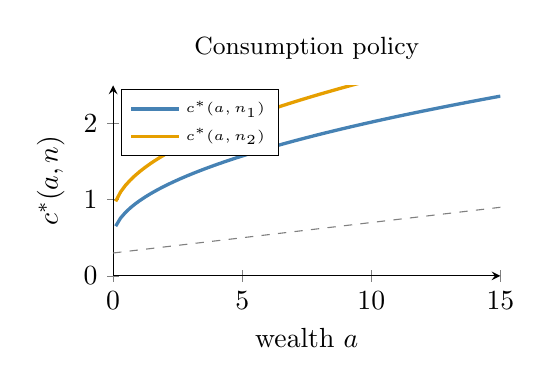
\begin{tikzpicture}
\begin{axis}[
    width=6.5cm, height=4cm,
    xlabel={wealth $a$}, ylabel={$c^*(a,n)$},
    xmin=0, xmax=15, ymin=0, ymax=2.5,
    axis lines=left,
    title={\small Consumption policy},
    legend style={at={(0.02,0.98)}, anchor=north west, font=\tiny},
]
\addplot[softblue, very thick, domain=0.1:15, samples=80]
    {0.5 + 0.8*sqrt(x) * 0.6};
\addlegendentry{$c^*(a, n_1)$}
\addplot[softorange, very thick, domain=0.1:15, samples=80]
    {0.8 + 0.8*sqrt(x) * 0.7};
\addlegendentry{$c^*(a, n_2)$}
% 45-degree reference
\addplot[dashed, gray, thin, domain=0:15] {0.04*x + 0.3};
\end{axis}
\end{tikzpicture}
\end{center}

\column{0.48\textwidth}
\begin{center}
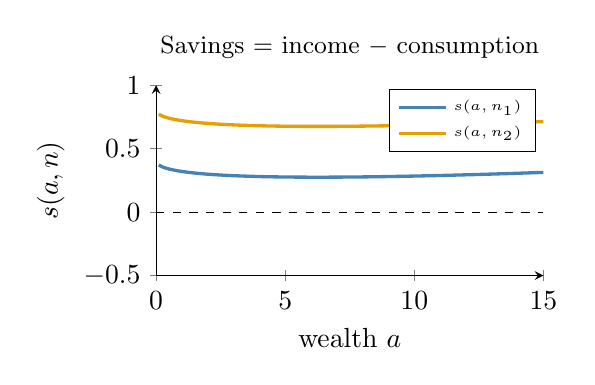
\begin{tikzpicture}
\begin{axis}[
    width=6.5cm, height=4cm,
    xlabel={wealth $a$}, ylabel={$s(a,n)$},
    xmin=0, xmax=15, ymin=-0.5, ymax=1.0,
    axis lines=left,
    title={\small Savings $=$ income $-$ consumption},
    legend style={at={(0.98,0.98)}, anchor=north east, font=\tiny},
]
\addplot[softblue, very thick, domain=0.1:15, samples=80]
    {0.4 - 0.2*sqrt(x)*0.5 + 0.02*x};
\addlegendentry{$s(a, n_1)$}
\addplot[softorange, very thick, domain=0.1:15, samples=80]
    {0.8 - 0.2*sqrt(x)*0.5 + 0.02*x};
\addlegendentry{$s(a, n_2)$}
\addplot[dashed, black, thin, domain=0:15] {0};
\end{axis}
\end{tikzpicture}
\end{center}
\end{columns}

\vspace{0.1em}
\begin{itemize}\itemsep1pt
    \item Low-income agents near $\ubar{a}$: savings near zero, often constrained
    \item High-income agents: positive savings $\Rightarrow$ accumulate wealth
    \item \emphc{Precautionary savings}: more saving than in the certainty benchmark
\end{itemize}
\end{frame}

% --- Slide: HJB with Aggregate Shocks ---
\begin{frame}{HJB with Aggregate Shocks (Krusell--Smith)}
\small
When aggregate TFP $Z_t$ follows $dZ_t = \eta(\bar{Z} - Z_t)\ud t + \sigma^z \ud B_t^0$,
the value function depends on the \emphc{entire wealth distribution} $g$: $V = V(a, n, z, g)$.
The \textbf{HJB} becomes:
\vspace{-0.3em}
\begin{multline*}
\rho V(a,n,z,g) = \max_c\Big\{u(c) + \partial_a V\cdot(w(z,g)\,n + r(z,g)\,a - c)\\
+ \lambda(n)\big(V(a,\hat{n},z,g) - V(a,n,z,g)\big)\\
+ \partial_z V\cdot\mu^z(z) + \tfrac{1}{2}(\sigma^z)^2\,\partial_{zz}V + \sum_j \int_{\ubar{a}}^\infty \frac{\delta V}{\delta g_j}(a, n_j, z, g)(y) \cdot \mu^g_j(y,z,g) \ud y \Big\}
\end{multline*}
\vspace{-0.8em}
\begin{alertblock}{\small The Curse of Dimensionality}
\small
$g$ is \emphc{infinite-dimensional}. Read $\frac{\delta V}{\delta g_j}(\cdot)(y)$ as the Gâteaux/functional derivative: how $V$ changes when a small bump of mass is added at wealth~$y$ in productivity-state~$j$. After a finite-dimensional approximation of $g$ (cf.\ Deck 2 \textit{Three Approximations}), it collapses to ordinary partials $\partial V/\partial\hat\varphi_i$. This makes the PDE intractable by standard methods $\Rightarrow$ \emphc{deep learning} (EMINNs --- Deck 2).
\end{alertblock}
\end{frame}

% --- Slide: Coupling HJB and KFE ---
\begin{frame}{The Coupled HJB--KFE System}
\begin{center}
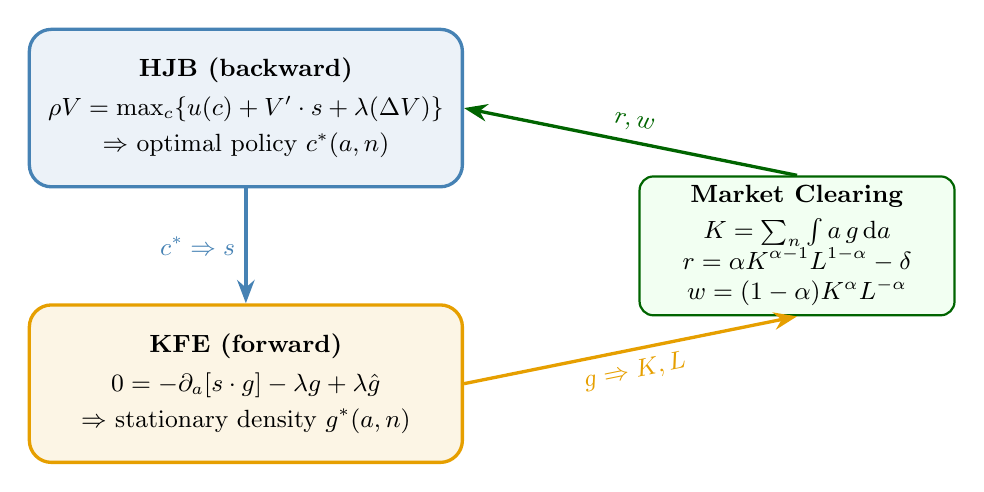
\begin{tikzpicture}[
    box/.style={rectangle, rounded corners=8pt, draw, very thick, minimum width=5.5cm, minimum height=2cm, align=center, font=\small},
    pricebox/.style={rectangle, rounded corners=5pt, draw=darkgreen, thick, fill=green!5, minimum width=4cm, minimum height=1cm, align=center, font=\small},
    arrow/.style={-Stealth, very thick}
]
\node[box, fill=softblue!10, draw=softblue] (hjb) at (0,2.5) {\textbf{HJB (backward)}\\[3pt]
    $\rho V = \max_c\{u(c) + V'\cdot s + \lambda(\Delta V)\}$\\[2pt]
    $\Rightarrow$ optimal policy $c^*(a,n)$};

\node[box, fill=softorange!10, draw=softorange] (kfe) at (0,-1) {\textbf{KFE (forward)}\\[3pt]
    $0 = -\partial_a[s\cdot g] - \lambda g + \lambda \hat{g}$\\[2pt]
    $\Rightarrow$ stationary density $g^*(a,n)$};

\node[pricebox] (mc) at (7,0.75) {\textbf{Market Clearing}\\[2pt]
    $K = \sum_n\int a\,g\ud a$\\
    $r = \alpha K^{\alpha-1}L^{1-\alpha} - \delta$\\
    $w = (1-\alpha)K^\alpha L^{-\alpha}$};

\draw[arrow, softblue] (hjb.south) -- node[left, font=\small] {$c^* \Rightarrow s$} (kfe.north);
\draw[arrow, softorange] (kfe.east) -- node[below, font=\small, sloped] {$g \Rightarrow K, L$} (mc.south);
\draw[arrow, darkgreen] (mc.north) -- node[above, font=\small, sloped] {$r, w$} (hjb.east);
\end{tikzpicture}
\end{center}

\vspace{0.1em}
\textbf{Solution method}: iterate until convergence (Aiyagari, no aggregate shocks):
\begin{enumerate}\itemsep1pt
    \item Guess $r$ $\to$ solve HJB for $V, c^*$ $\to$ solve KFE for $g^*$ $\to$ compute $K$ $\to$ update $r$
\end{enumerate}
\end{frame}

% ============================================================================
% PART V: COMPETITIVE EQUILIBRIUM
% ============================================================================

\section{Competitive Equilibrium}

\begin{frame}{}
\vfill
\begin{center}
{\Huge \textcolor{uzhblue}{\textbf{Part IV}}}\\[12pt]
{\LARGE Competitive Equilibrium}\\[6pt]
{\large Aiyagari (1994) and Krusell--Smith (1998)}
\end{center}
\vfill
\end{frame}

% --- Slide: Environment ---
\begin{frame}{Setting: Agents and Preferences}
\small
\begin{itemize}\itemsep1pt
    \item \textbf{Continuous time}, infinite horizon, one consumption good
    \item \textbf{Population}: continuum of agents $i \in I = [0,1]$
    \item \textbf{Preferences}: $\E{\int_0^\infty e^{-\rho t}\,u(c_t^i)\ud t}$, \; $u(c) = \frac{c^{1-\gamma}}{1-\gamma}$
    \item \textbf{Labor endowment}: $n_t^i \in \{n_1, n_2\}$ follows a CTMC:
    \begin{itemize}\itemsep0pt
        \item $n_1 \to n_2$ with Poisson intensity $\lambda_1$; \; $n_2 \to n_1$ with intensity $\lambda_2$
    \end{itemize}
\end{itemize}

\vspace{0.1em}
\begin{center}
\renewcommand{\arraystretch}{1.0}
\begin{tabular}{ll}
\toprule
\textbf{Parameter} & \textbf{Interpretation} \\
\midrule
$\rho$ & Discount rate \\
$\gamma$ & Risk aversion (inverse EIS) \\
$n_1 < n_2$ & Low / high labor productivity \\
$\lambda_1, \lambda_2$ & Transition intensities \\
\bottomrule
\end{tabular}
\end{center}
\end{frame}

% --- Slide: Production ---
\begin{frame}{Production Technology}
\small
\textbf{Representative firm}: $Y_t = e^{Z_t} F(K_t, L_t) = e^{Z_t} K_t^\alpha L_t^{1-\alpha}$

\begin{itemize}\itemsep1pt
    \item $K_t, L_t$: capital and labor hired at time $t$
    \item $F$: CRS production function (Cobb--Douglas)
    \item \textbf{Aiyagari} (1994): $Z_t = \bar{Z}$ constant $\Rightarrow$ no aggregate risk
    \item \textbf{Krusell--Smith} (1998): $Z_t$ follows OU: $dZ_t = \eta(\bar{Z} - Z_t)\ud t + \sigma^z\ud B_t^0$
\end{itemize}

\vspace{0.1em}
\textbf{Additional assumptions:}
\begin{itemize}\itemsep1pt
    \item Consumption $\leftrightarrow$ capital conversion at $1:1$ ratio
    \item Capital depreciates at rate $\delta$
\end{itemize}
\end{frame}

% --- Slide: Markets ---
\begin{frame}{Markets}
\small
\begin{itemize}\itemsep2pt
    \item \textbf{Incomplete financial markets}:
    \begin{itemize}\itemsep2pt
        \item Agents \emphc{cannot insure} idiosyncratic income risk
        \item Instead, agents ``save and borrow claims on capital''
        \item $a_t$: agent's claim on capital stock
        \item \emphc{Borrowing constraint}: $a_t \geq \ubar{a} > -\infty$
    \end{itemize}
    \item \textbf{Competitive capital market} with rental rate $r_t$:
    \[
    \text{Clearing:} \quad \int_I a_t^i \ud i = K_t
    \]
    \item \textbf{Competitive labor market} with wage $w_t$:
    \[
    \text{Clearing:} \quad \int_I n_t^i \ud i = L_t
    \]
    \item \textbf{Goods market}: clears by Walras's Law
\end{itemize}

\vspace{0.1em}
{\scriptsize If $a_t<0$, interpret this as borrowing from a frictionless intermediary that pools deposits and finances capital.}
\end{frame}

% --- Slide: Firm Problem ---
\begin{frame}{Firm Problem}
\small
The representative firm solves:
\[
\max_{K_t, L_t} \left\{e^{Z_t}F(K_t, L_t) - (r_t + \delta)K_t - w_t L_t\right\}
\]

\textbf{First-order conditions:}
\begin{align*}
r_t &= e^{Z_t}\,\partial_K F(K_t, L_t) - \delta = \alpha e^{Z_t} K_t^{\alpha-1}L_t^{1-\alpha} - \delta \\[6pt]
w_t &= e^{Z_t}\,\partial_L F(K_t, L_t) = (1-\alpha)e^{Z_t}K_t^\alpha L_t^{-\alpha}
\end{align*}

\vspace{0.2em}
Prices are \emphc{functions of the aggregate state}:
\[
q_t = \begin{bmatrix} r_t \\ w_t \end{bmatrix} = Q(Z_t, g_t)
\]
where $K_t = \sum_{j \in \{1,2\}} \int a\,g_t(a, n_j)\ud a$.

\vspace{0.3em}
{\small Having explicit expressions for prices in terms of $(Z_t, g_t)$ makes the problem tractable.}
\end{frame}

% --- Slide: KFE in Equilibrium ---
\begin{frame}{Kolmogorov Forward Equation in Equilibrium}
\small
Given stochastic processes $\{c^*, \tilde{r}, \tilde{w}\}$, at time $t > 0$, on $(\ubar{a}, \infty)$, the \emphc{density} $g_t(a,n)$ satisfies the KFE:

\[
\boxed{\partial_t g_t(a,n) = -\partial_a\!\Big[(\tilde{w}_t n + \tilde{r}_t a - c_t^*)\,g_t(a,n)\Big] - \lambda(n)\,g_t(a,n) + \lambda(\hat{n})\,g_t(a,\hat{n})}
\]

\vspace{0.2em}
\textbf{Observations:}
\begin{itemize}\itemsep2pt
    \item Why does the KFE \emphc{not} have $dB_t^0$?
    \begin{itemize}
        \item Idiosyncratic shocks wash out at the population level (LLN)
        \item But with aggregate shocks (KS): $g_t$ is stochastic via prices
    \end{itemize}
    \item $g_t(a,n)$ is still stochastic in equilibrium since $r$ and $w$ depend on $\mathcal{F}_t^0$
    \item Low-income agents ``stuck'' at borrowing constraint $\Rightarrow$ boundary atom in $g_t$
    \item Technical: need \emphc{measure-valued} solution (Achdou et al., 2022)
\end{itemize}
\end{frame}

% --- Slide: Equilibrium Definition ---
\begin{frame}{Definition: Rational Expectations Equilibrium}
\small
\begin{block}{Definition (Rational Expectations Equilibrium)}
\small
Given initial density $g_0$, an \emphc{equilibrium} is $\mathcal{F}_t^0$-adapted processes $\{c_t^i, g_t, z_t, q_t := [r_t, w_t]\}$ such that:

\begin{enumerate}\itemsep1pt
    \item \textbf{Household optimality}: Given price belief $\tilde{q}$, $c_t^i$ solves HJB.
    \item \textbf{Firm optimality}: $r_t = e^{Z_t}\partial_K F - \delta$, \; $w_t = e^{Z_t}\partial_L F$
    \item \textbf{Market clearing}:
    $K_t = \sum_{j} \int a\,g_t(a,n_j)\ud a$, \; $L = \sum_{j} \int n_j\,g_t(a,n_j)\ud a$
    \item \textbf{Belief consistency}: $\tilde{q} = q$ \quad (beliefs $=$ actual prices)
\end{enumerate}
\end{block}
\end{frame}

% --- Slide: Stationary Equilibrium ---
\begin{frame}{Derivation Map: Model $\Rightarrow$ HJB $\Rightarrow$ KFE $\Rightarrow$ Equilibrium}
\footnotesize
\textbf{Step 1 (household control problem):}
\[
da_t=(w n_t+r a_t-c_t)\ud t,\qquad n_t\in\{n_1,n_2\}\ \text{(Poisson switching)}.
\]

\vspace{-0.2em}
\textbf{Step 2 (HJB + FOC):}
\[
\rho V(a,n)=\max_c\left\{u(c)+V_a(a,n)\,[w n+r a-c]+\lambda(n)\big(V(a,\hat n)-V(a,n)\big)\right\},
\]
\[
u'(c^*(a,n))=V_a(a,n),\qquad s(a,n):=w n+r a-c^*(a,n).
\]

\vspace{-0.2em}
\textbf{Step 3 (KFE induced by optimal drift $s$):}
\[
0=-\partial_a[s(a,n)g^*(a,n)]-\lambda(n)g^*(a,n)+\lambda(\hat n)g^*(a,\hat n).
\]

\vspace{-0.2em}
\textbf{Step 4 (general equilibrium closure, Aiyagari):}
\[
K=\sum_n\int a\,g^*(a,n)\ud a,\qquad L=\sum_n\int n\,g^*(a,n)\ud a,
\]
\[
r=\alpha K^{\alpha-1}L^{1-\alpha}-\delta,\qquad w=(1-\alpha)K^\alpha L^{-\alpha}.
\]

\vspace{0.1em}
\textbf{Fixed point}: iterate on $(r,w)$ until household supply and firm demand are consistent.
\end{frame}

% --- Slide: Three Equilibrium Notions ---
\begin{frame}{Three Notions of Equilibrium}
\small
{\small Following Sargent (1999, 2008):}

\vspace{0.2em}
\begin{enumerate}\itemsep3pt
    \item \textbf{Rational expectations equilibrium}
    \begin{itemize}
        \item Agents' perceived law of motion $=$ true law of motion
        \item Even for data that would \emph{never} be generated on the equilibrium path
    \end{itemize}

    \item \textbf{Self-confirming belief equilibrium}
    \begin{itemize}
        \item Agents' model is the best statistical fit to data generated by the economy
        \item Agents would never reject their model based on observed data
        \item But may have incorrect off-equilibrium beliefs
    \end{itemize}

    \item \textbf{Optimal misspecified belief equilibrium}
    \begin{itemize}
        \item Agents use an optimally chosen (but possibly wrong) model
        \item Robust decision-making under model uncertainty
    \end{itemize}
\end{enumerate}

\vspace{0.3em}
{\small In this course: we focus on \emphc{rational expectations}. But note: neural network ``solvers'' can naturally accommodate bounded rationality (approximate equilibria).}
\end{frame}

% --- Slide: Huggett Economic Intuition ---
\begin{frame}[shrink=2]{Huggett (1993): Economic Mechanism}
\small
\begin{columns}[T]
\column{0.53\textwidth}
\textbf{Environment}
\begin{itemize}\itemsep2pt
    \item Endowment economy with idiosyncratic income $y_t\in\{y_1,y_2\}$.
    \item Incomplete markets: only one risk-free bond $b_t$.
    \item Borrowing limit $b_t\ge \ubar b$.
    \item Bond is in zero net supply.
\end{itemize}

\textbf{Household trade-off}
\begin{itemize}\itemsep2pt
    \item Low income state: wants to borrow to smooth consumption.
    \item High income state: saves for self-insurance.
    \item Constraint creates a mass of constrained agents at $\ubar b$.
\end{itemize}

\column{0.44\textwidth}
\textbf{How equilibrium price is determined}
\begin{itemize}\itemsep2pt
    \item For candidate return $q$, solve HJB $\Rightarrow$ policy $s(b,y)$.
    \item Propagate policy through KFE $\Rightarrow$ stationary density $g^*(b,y)$.
    \item Compute aggregate bond demand:
    \[
    B^s(q)=\sum_y\int_{\ubar b}^{\infty} b\,g^*(b,y)\ud b.
    \]
    \item Equilibrium return: $q^*$ such that $B^s(q^*)=0$.
\end{itemize}
\vspace{0.1em}
\textbf{Implication}: the risk-free rate is pinned down by precautionary self-insurance demand, not by a production FOC.
\end{columns}
\end{frame}

% --- Slide: Aiyagari Economic Intuition I ---
\begin{frame}[shrink=2]{Aiyagari (1994): Economic Mechanism I}
\small
\begin{columns}[T]
\column{0.53\textwidth}
\textbf{What changes vs.\ Huggett}
\begin{itemize}\itemsep2pt
    \item Add a representative firm with Cobb--Douglas production.
    \item Household asset is now a claim on aggregate capital $a_t$.
    \item Same incomplete insurance and borrowing constraint logic.
    \item Aggregate capital is \emphc{endogenously positive}: $K>0$.
\end{itemize}

\textbf{Supply side (households)}
\begin{itemize}\itemsep2pt
    \item For given $(r,w)$, HJB gives policy $s(a,z)$.
    \item KFE gives density $g^*(a,z)$.
    \item Capital supplied by households:
    $K^s(r)=\sum_z\int_{\ubar a}^{\infty} a\,g^*(a,z)\ud a$.
\end{itemize}

\column{0.44\textwidth}
\textbf{Intuition}
\begin{itemize}\itemsep2pt
    \item Low productivity states generate demand for insurance via saving.
    \item High productivity states accumulate assets.
    \item With many uninsured households, aggregate saving pressure is high.
    \item This pushes the equilibrium return on capital downward.
\end{itemize}
\end{columns}
\end{frame}

% --- Slide: Aiyagari Economic Intuition II ---
\begin{frame}[shrink=2]{Aiyagari (1994): Economic Mechanism II}
\small
\textbf{General-equilibrium closure}
\begin{columns}[T]
\column{0.50\textwidth}
\textbf{Firm demand for capital}
\[
r=\alpha K^{\alpha-1}L^{1-\alpha}-\delta
\]
\[
w=(1-\alpha)K^\alpha L^{-\alpha}
\]
These conditions imply a decreasing capital-demand schedule $K^d(r)$.

\vspace{0.3em}
\textbf{Household capital supply}
\[
K^s(r)=\sum_z\int_{\ubar a}^{\infty} a\,g^*(a,z)\ud a,
\]
where $g^*$ is the stationary density induced by optimal savings.

\column{0.46\textwidth}
\textbf{Equilibrium condition}
\[
K^s(r^*)=K^d(r^*),\qquad w^*=w(r^*).
\]

\begin{block}{Economic interpretation}
\small
Aiyagari is a full GE model: prices are jointly determined by
\begin{itemize}\itemsep1pt
    \item household self-insurance behavior (asset supply), and
    \item firm marginal productivity (asset demand).
\end{itemize}
\end{block}
\end{columns}
\end{frame}

% --- Slide: Huggett Model ---
\begin{frame}{Huggett (1993): Formal Stationary PDE System}
\scriptsize
\textbf{Primitives}: endowment economy, $b_t\ge\ubar b$, $y_t\in\{y_1,y_2\}$ with Poisson switching.  Bonds pay instantaneous return $r$ (price-vs-return convention: $r$, not a bond price $q$).
\[
db_t=(r\,b_t+y_t-c_t)\ud t,\qquad
\max_{\{c_t\}} \E{}\!\left[\int_0^\infty e^{-\rho t}u(c_t)\ud t\right].
\]

\textbf{HJB} (state $y$):
\[
\rho V=\max_c\{u(c)+V_b(rb+y-c)+\lambda(y)(V(b,\hat y)-V(b,y))\},\quad
u'(c^*)=V_b,\quad s=rb+y-c^*.
\]

\textbf{KFE} on $(\ubar b,\infty)$:
\[
0=-\partial_b[s(b,y)g^*(b,y)]-\lambda(y)g^*(b,y)+\lambda(\hat y)g^*(b,\hat y),
\]
\[
J(\ubar b,y)=s(\ubar b,y)g^*(\ubar b,y)=0,\qquad
\sum_{y}\int_{\ubar b}^{\infty}g^*(b,y)\ud b=1.
\]

\textbf{Bond market clearing}:
\[
\sum_{y}\int_{\ubar b}^{\infty} b\,g^*(b,y)\ud b=0.
\]
Unknowns: $(V,g^*,q)$.
\end{frame}

% --- Slide: Aiyagari Model ---
\begin{frame}{Aiyagari (1994): Formal Stationary PDE System}
\footnotesize
\textbf{Production side} (no aggregate shocks):
\[
Y=K^\alpha L^{1-\alpha},\qquad
r=\alpha K^{\alpha-1}L^{1-\alpha}-\delta,\qquad
w=(1-\alpha)K^\alpha L^{-\alpha}.
\]

\vspace{0.1em}
\textbf{Household problem}:
\[
\max_{\{c_t\}} \E{}\!\left[\int_0^\infty e^{-\rho t}u(c_t)\ud t\right],\qquad
da_t=(w z_t+r a_t-c_t)\ud t,\qquad a_t\ge \ubar a,\quad z_t\in\{z_1,z_2\}.
\]

\vspace{0.1em}
\textbf{HJB}:
\[
\rho V(a,z)=\max_c\left\{u(c)+V_a(a,z)\,[w z+r a-c]+\lambda(z)\big(V(a,\hat z)-V(a,z)\big)\right\},
\]
\[
u'(c^*)=V_a,\qquad s(a,z):=w z+r a-c^*(a,z).
\]

\vspace{0.1em}
\textbf{KFE} on $(\ubar a,\infty)$:
\[
0=-\partial_a\!\big[s(a,z)g^*(a,z)\big]-\lambda(z)g^*(a,z)+\lambda(\hat z)g^*(a,\hat z).
\]

\vspace{0.1em}
\textbf{Market clearing \& normalization:}
\[
K=\sum_{z}\int_{\ubar a}^{\infty} a\,g^*(a,z)\ud a,\qquad
L=\sum_{z}\int_{\ubar a}^{\infty} z\,g^*(a,z)\ud a,\qquad
\sum_{z}\int_{\ubar a}^{\infty} g^*(a,z)\ud a=1.
\]
Unknowns: $(V,g^*,r,w,K)$ (or $(V,g^*,r)$ with $w=w(r)$).
\end{frame}

% --- Slide: Huggett vs Aiyagari ---
\begin{frame}{Huggett vs.\ Aiyagari: Key Differences}
\small
\begin{center}
\renewcommand{\arraystretch}{1.1}
\begin{tabular}{lcc}
\toprule
& \textbf{Huggett (1993)} & \textbf{Aiyagari (1994)} \\
\midrule
Economy & Endowment & Production ($Y = K^\alpha L^{1-\alpha}$) \\
Asset & Bond $b$ & Capital claim $a$ \\
Supply & Zero net ($\int b = 0$) & Positive ($\int a = K > 0$) \\
Price & Bond return $q$ & Interest rate $r$, wage $w$ \\
Clearing & $\int b\,g\ud b = 0$ & $\int a\,g\ud a = K(r)$ \\
\bottomrule
\end{tabular}
\end{center}

\vspace{0.1em}
\textbf{How the distributions differ:}
\begin{columns}[T]
\column{0.48\textwidth}
\textbf{Huggett:}
\begin{itemize}\itemsep0pt
    \item Wealth centered around $0$ (zero net supply)
    \item Large mass at borrowing constraint
    \item Symmetric-ish with constrained left tail
\end{itemize}

\column{0.48\textwidth}
\textbf{Aiyagari:}
\begin{itemize}\itemsep0pt
    \item Wealth shifted right ($K > 0$)
    \item Long right tail (wealthy agents)
    \item Smaller mass at constraint
\end{itemize}
\end{columns}
\end{frame}

% --- Slide: Distribution Comparison ---
\begin{frame}{Wealth Distributions: Huggett vs.\ Aiyagari}
\small
\begin{columns}[T]
\column{0.48\textwidth}
\begin{center}
\textbf{Huggett (1993)}\\[2pt]
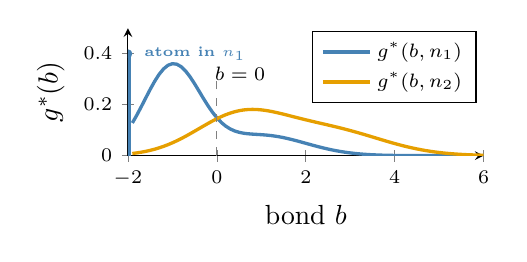
\begin{tikzpicture}
\begin{axis}[
    width=6.1cm, height=3.2cm,
    xlabel={bond $b$}, ylabel={$g^*(b)$},
    xmin=-2, xmax=6, ymin=0, ymax=0.5,
    axis lines=left,
    tick label style={font=\scriptsize},
    label style={font=\normalsize},
    legend style={at={(0.98,0.98)}, anchor=north east, font=\scriptsize},
]
% Low income (n_1) -- smooth density on (b_lower, infty)
\addplot[softblue, very thick, domain=-1.9:6, samples=80]
    {0.35*exp(-(x+1)^2/0.8) + 0.08*exp(-(x-1)^2/2)};
\addlegendentry{$g^*(b, n_1)$}
% High income (n_2) -- no atom at the constraint
\addplot[softorange, very thick, domain=-1.9:6, samples=80]
    {0.15*exp(-(x-0.5)^2/2) + 0.1*exp(-(x-2.5)^2/3)};
\addlegendentry{$g^*(b, n_2)$}
% Dirac atom at borrowing constraint -- carried by the constrained (low-income) type only
\draw[softblue, line width=2.2pt] (axis cs:-2,0) -- (axis cs:-2,0.40);
\fill[softblue] (axis cs:-2,0.40) circle (1.6pt);
\node[softblue, font=\tiny\bfseries, anchor=west]
    at (axis cs:-1.85,0.40) {atom in $n_1$};
\draw[dashed, gray] (axis cs:0,0) -- (axis cs:0,0.3);
\node[font=\scriptsize] at (axis cs:0.52,0.32) {$b=0$};
\end{axis}
\end{tikzpicture}
\end{center}
{\scriptsize Net supply $= 0$: mean wealth $\approx 0$.}

\column{0.48\textwidth}
\begin{center}
\textbf{Aiyagari (1994)}\\[2pt]
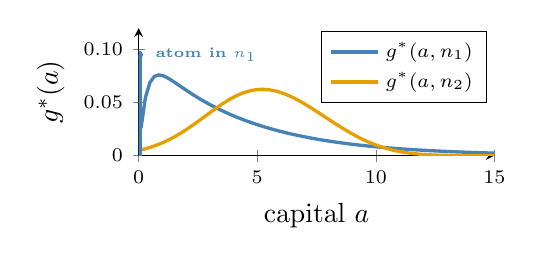
\begin{tikzpicture}
\begin{axis}[
    width=6.1cm, height=3.2cm,
    xlabel={capital $a$}, ylabel={$g^*(a)$},
    xmin=0, xmax=15, ymin=0, ymax=0.12,
    axis lines=left,
    scaled y ticks=false,
    ytick={0,0.05,0.10},
    yticklabels={0,0.05,0.10},
    tick label style={font=\scriptsize},
    label style={font=\normalsize},
    legend style={at={(0.98,0.98)}, anchor=north east, font=\scriptsize},
]
% Low income (n_1) -- smooth density on (0, infty)
\addplot[softblue, very thick, domain=0.1:15, samples=80]
    {0.09*exp(-0.25*(x-0.5)) * (1 - exp(-3*x))};
\addlegendentry{$g^*(a, n_1)$}
% High income (n_2) -- no atom at the constraint
\addplot[softorange, very thick, domain=0.1:15, samples=80]
    {0.06*exp(-(x-5)^2/10) + 0.01*exp(-(x-8)^2/6)};
\addlegendentry{$g^*(a, n_2)$}
% Dirac atom at borrowing constraint -- carried by the constrained (low-income) type only
\draw[softblue, line width=2.2pt] (axis cs:0,0) -- (axis cs:0,0.095);
\fill[softblue] (axis cs:0,0.095) circle (1.6pt);
\node[softblue, font=\tiny\bfseries, anchor=west]
    at (axis cs:0.3,0.095) {atom in $n_1$};
\end{axis}
\end{tikzpicture}
\end{center}
{\scriptsize $K>0$: mean wealth is positive with a right tail.}
\end{columns}

\end{frame}

% --- Slide: Why This Matters - HANK ---
\begin{frame}[shrink=2]{Why This Matters: HANK and Modern Macro}
\small
The Aiyagari/Krusell--Smith framework is the \emphc{backbone of HANK}:

\vspace{0.1em}
\begin{columns}[T]
\column{0.48\textwidth}
\textbf{Heterogeneous Agent New Keynesian:}
\begin{itemize}\itemsep2pt
    \item Kaplan, Moll \& Violante (2018, \emph{AER})
    \item Replace representative agent with Aiyagari economy
    \item Add nominal rigidities
    \item Result: monetary policy affects consumption \emphc{heterogeneously}
\end{itemize}

\vspace{0.3em}
\textbf{Applications:}
\begin{itemize}\itemsep2pt
    \item Fiscal stimulus (who spends?)
    \item Inequality dynamics
    \item Wealth taxation
    \item COVID-19 policy responses
\end{itemize}

\column{0.48\textwidth}
\textbf{Key insight from HANK:}

\vspace{0.2em}
\begin{center}
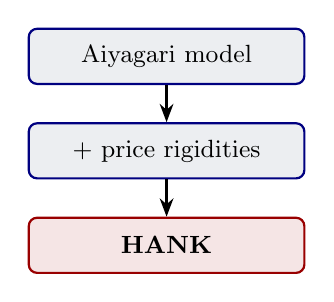
\begin{tikzpicture}[
    box/.style={rectangle, rounded corners=3pt, draw=uzhblue, thick, fill=uzhgreylight, minimum width=3.5cm, minimum height=0.7cm, align=center, font=\small}
]
\node[box] (aiy) at (0,2.4) {Aiyagari model};
\node[box] (nk) at (0,1.2) {+ price rigidities};
\node[box, draw=harvardcrimson, fill=harvardcrimson!10] (hank) at (0,0) {\textbf{HANK}};
\draw[-Stealth, thick] (aiy) -- (nk);
\draw[-Stealth, thick] (nk) -- (hank);
\end{tikzpicture}
\end{center}

\vspace{0.1em}
{\scriptsize ``These building blocks are essential for modern macro.''}
\end{columns}
\end{frame}

% ============================================================================
% PART VI: THE MASTER EQUATION
% ============================================================================

\section{The Master Equation}

\begin{frame}{}
\vfill
\begin{center}
{\Huge \textcolor{uzhblue}{\textbf{Part V}}}\\[12pt]
{\LARGE The Master Equation}\\[6pt]
{\large From Coupled System to Single PDE}
\end{center}
\vfill
\end{frame}

% --- Slide: Recursive Representation ---
\begin{frame}{Recursive Representation of Equilibrium}
\footnotesize
\textbf{States}: individual $x=(a,n)$, aggregate $(z,g)$; value function $V(x,z,g)$.

\vspace{0.1em}
Given a belief drift $\hat\mu^g$, the household HJBE is
\[
\begin{aligned}
0=\max_c\Big\{&-\rho V + u(c) + V_a\,[w(z,g)n+r(z,g)a-c] + \lambda(n)\big(V(a,\hat n,z,g)-V(a,n,z,g)\big)\\
&+V_z\,\mu^z(z)+\tfrac12(\sigma^z)^2V_{zz}
+\sum_{j\in\{1,2\}}\int_{\ubar a}^{\infty}
\frac{\delta V}{\delta g_j}(a,n,z,g)(y)\,\hat\mu^g_j(y,z,g)\ud y
\Big\}.
\end{aligned}
\]

\vspace{-0.2em}
For $c^*(a,n,z,g;\hat\mu^g)$, the density drift is
\[
\mu^g_j(a,z,g)= -\partial_a\!\big[(w(z,g)n_j+r(z,g)a-c^*_j(a,z,g))\,g_j(a)\big]
-\lambda_j g_j(a)+\lambda_{\hat j} g_{\hat j}(a).
\]
\textbf{Equilibrium consistency}: $\hat\mu^g=\mu^g$.
\end{frame}

% --- Slide: The Master Equation ---
\begin{frame}{The Master Equation}
\footnotesize
\emphc{Key idea}: Substitute KFE, market clearing, and belief consistency \emphc{into} the HJBE.
Result: \emphc{one PDE} characterizing the equilibrium value function:

\vspace{0.1em}
\begin{block}{Master Equation}
\footnotesize
\vspace{-0.2em}
\begin{multline*}
0 = -\rho V(a,n,z,g) + u(c^*) + V_a\,[w(z,g)n+r(z,g)a-c^*] \\
+ \lambda(n)\!\left(V(a,\hat n,z,g)-V(a,n,z,g)\right)
+ V_z\,\mu^z(z) + \tfrac12(\sigma^z)^2V_{zz} \\
+ \sum_{j\in\{1,2\}}\int_{\ubar a}^{\infty}
\frac{\delta V}{\delta g_j}(a,n,z,g)(y)\,\mu^g_j(y,z,g)\ud y
\;=:\;\mathcal{L}V.
\end{multline*}
\vspace{-0.2em}
\end{block}

where $c^*$ satisfies $u'(c^*) = \partial_a V(a,n,z,g)$.

\vspace{0.2em}
\begin{center}
\colorbox{uzhgreylight}{\parbox{0.6\textwidth}{\centering\small
\textbf{``One equation to rule them all''}\\
HJB + KFE + market clearing = master equation}}
\end{center}
\end{frame}

% --- Slide: Envelope Condition Version ---
\begin{frame}{The Envelope Condition: Working with $W := \partial_a V$}
\small
\textbf{Practical insight} (Gu, Lauriere, Merkel \& Payne, 2024):
It is easier to work with $W(a,l,z,g) := \partial_a V(a,l,z,g)$ rather than $V$ itself.

\textbf{Why?} Because $W$ \emphc{directly gives the consumption policy}:
$u'(c^*(a,n,z,g)) = W(a,n,z,g) \;\Leftrightarrow\; c^* = W^{-1/\gamma}$

The \textbf{master equation for $W$} (using the envelope theorem):
\[
\boxed{0 = (r(z,g) - \rho)\,W + \underbrace{\mathcal{L}_x W}_{\text{individual}} + \underbrace{\mathcal{L}_z W}_{\text{aggregate TFP}} + \underbrace{\mathcal{L}_g W}_{\text{distribution}} =: \mathcal{L}W}
\]
where:
\begin{itemize}\itemsep2pt
    \item $\mathcal{L}_x W$: individual state dynamics (savings, income switching)
    \item $\mathcal{L}_z W$: aggregate TFP dynamics ($\partial_z W \cdot \mu^z + \frac{1}{2}(\sigma^z)^2\partial_{zz}W$)
    \item $\mathcal{L}_g W$: distribution dynamics (functional derivative w.r.t.\ $g$)
\end{itemize}
\end{frame}

% --- Slide: Why Master Equation ---
\begin{frame}[shrink=2]{Why the Master Equation?}
\small
\begin{columns}[T]
\column{0.48\textwidth}
\textbf{Advantages:}
\begin{itemize}\itemsep2pt
    \item[\textcolor{darkgreen}{\ding{51}}] \emphc{Single PDE} instead of coupled HJB + KFE + MC
    \item[\textcolor{darkgreen}{\ding{51}}] No separate market clearing step
    \item[\textcolor{darkgreen}{\ding{51}}] Amenable to \emphc{neural network approximation}:\\
    parameterize $V$ or $W$ by a deep net
    \item[\textcolor{darkgreen}{\ding{51}}] Auto-differentiation computes all derivatives (including functional derivative w.r.t.\ $g$)
\end{itemize}

\column{0.48\textwidth}
\textbf{Challenges:}
\begin{itemize}\itemsep2pt
    \item[\textcolor{darkred}{\ding{55}}] \emphc{Infinite-dimensional}: functional derivative $\frac{\delta V}{\delta g_j}$
    \item[\textcolor{darkred}{\ding{55}}] Need finite-dimensional approximation of $g$
    \item[\textcolor{darkred}{\ding{55}}] Training can be unstable (``bad approximate solutions'')
    \item[\textcolor{darkred}{\ding{55}}] No convergence guarantees
\end{itemize}
\end{columns}

\vspace{0.3em}
\begin{center}
\colorbox{uzhgreylight}{\parbox{0.85\textwidth}{\centering\small
\textbf{Deck 2 (after coffee)}: Three approaches to approximate $g$ in finite dimensions:\\
(1) Finite population, (2) Discrete state space, (3) Projection onto basis functions.\\
Then: solve the master equation with \emphc{EMINNs} (neural networks + auto-diff).
}}
\end{center}
\end{frame}

% --- Slide: Summary ---
\begin{frame}{Summary and Key Takeaways}
\begin{columns}[T]
\column{0.32\textwidth}
\begin{block}{Stochastic Calculus}
\centering\small
\vspace{0.2em}
Brownian motion, It\^o processes, It\^o's lemma, Poisson jumps --- the \emphc{language} of continuous-time models.
\vspace{0.2em}
\end{block}

\column{0.32\textwidth}
\begin{block}{KFE / Fokker--Planck}
\centering\small
\vspace{0.2em}
Tracks \emphc{density evolution} of a stochastic process. In economics: the wealth distribution.
\vspace{0.2em}
\end{block}

\column{0.32\textwidth}
\begin{block}{HJB + Equilibrium}
\centering\small
\vspace{0.2em}
Optimal control $\Rightarrow$ HJB. Coupled with KFE via savings policy. Master equation unifies all.
\vspace{0.2em}
\end{block}
\end{columns}

\vspace{0.3em}
\textbf{Next (numerical methods, after coffee):}
\begin{enumerate}\itemsep1pt
    \item Solve the coupled HJB+KFE by \emphc{finite differences} (benchmark)
    \item Solve the same system with \emphc{PINNs} (mesh-free, auto-diff)
    \item Solve the \emphc{master equation} with EMINNs (deep learning)
\end{enumerate}

\vspace{0.2em}
\begin{center}
\colorbox{uzhgreylight}{\parbox{0.5\textwidth}{\centering\small
\textbf{Coffee break!}\\
Back at 10:45 for numerical methods.}}
\end{center}
\end{frame}

% --- Slide: Theory-to-Code Bridge ---
\begin{frame}{From Theory to Code (Day 6 Notebook)}
\footnotesize
\textbf{Companion notebook:}
\begin{itemize}\itemsep2pt
    \item \texttt{lectures/day6/code/08\_Aiyagari\_Continuous\_Time\_FD\_and\_PINN\_PyTorch.ipynb}
\end{itemize}

\vspace{0.3em}
\textbf{Covers:}
\begin{itemize}\itemsep2pt
    \item Finite-difference solver for the Aiyagari HJB+KFE system
    \item PINN solver for the same equilibrium
    \item Comparison of stationary distributions, savings policies, and the equilibrium interest rate
\end{itemize}
\end{frame}

% --- Slide: References ---
\begin{frame}{References}
\tiny
\begin{columns}[T]
\column{0.48\textwidth}
\textbf{Foundational:}
\begin{itemize}\itemsep1pt
    \item Aiyagari, S.R.\ (1994). Uninsured Idiosyncratic Risk and Aggregate Saving. \emph{QJE} 109(3), 659--684.
    \item Bewley, T.\ (1980). The Optimum Quantity of Money. In \emph{Models of Monetary Economies}. Fed.\ Reserve Bank Minneapolis.
    \item Huggett, M.\ (1993). The Risk-Free Rate in HA Economies. \emph{JEDC} 17(5--6), 953--969.
    \item Krusell, P.\ \& Smith, A.A.\ (1998). Income and Wealth Heterogeneity. \emph{JPE} 106(5), 867--896.
\end{itemize}

\vspace{0.3em}
\textbf{Continuous-time formulations:}
\begin{itemize}\itemsep1pt
    \item Achdou, Y., Han, J., Lasry, J.-M., Lions, P.-L.\ \& Moll, B.\ (2022). Income and Wealth Distribution in Macroeconomics: A CT Approach. \emph{REStud} 89(1), 45--86.
    \item Gu, Z., Lauriere, M., Merkel, S.\ \& Payne, J.\ (2024). Global Solutions to Master Equations for CT HA Models. arXiv:2406.13726.
\end{itemize}

\column{0.48\textwidth}
\textbf{Mean field games:}
\begin{itemize}\itemsep1pt
    \item Lasry, J.-M.\ \& Lions, P.-L.\ (2007). Mean Field Games. \emph{Jpn.\ J.\ Math.}\ 2(1), 229--260.
\end{itemize}

\vspace{0.3em}
\textbf{HANK and applications:}
\begin{itemize}\itemsep1pt
    \item Kaplan, G., Moll, B.\ \& Violante, G.L.\ (2018). Monetary Policy According to HANK. \emph{AER} 108(3), 697--743.
    \item Gabaix, X., Lasry, J.-M., Lions, P.-L.\ \& Moll, B.\ (2016). The Dynamics of Inequality. \emph{Econometrica} 84(6), 2071--2111.
    \item Ahn, S., Kaplan, G., Moll, B., Winberry, T.\ \& Wolf, C.\ (2018). When Inequality Matters for Macro. \emph{NBER Macro Annual} 32(1), 1--75.
\end{itemize}

\vspace{0.3em}
\textbf{Deep learning for het.\ agent models:}
\begin{itemize}\itemsep1pt
    \item Fernandez-Villaverde, J., Hurtado, S.\ \& Nuno, G.\ (2023). Financial Frictions and the Wealth Distribution. \emph{Econometrica} 91(3), 869--901.
    \item Nuno, G.\ \& Moll, B.\ (2018). Social Optima in Economies with HA. \emph{RED} 28, 150--180.
\end{itemize}
\end{columns}
\end{frame}

% --- Slide: Questions ---
\begin{frame}{}
\begin{columns}[c]
\column{0.45\textwidth}
\begin{center}
{\Huge \textcolor{uzhblue}{\textbf{Questions?}}}

\vspace{1.0cm}
{\large Simon Scheidegger}\\[4pt]
{\small HEC, University of Lausanne}\\[4pt]
\url{https://sischei.github.io}

\vspace{0.6cm}
{\small Materials:~~\url{https://github.com/sischei/Deep_Learning_for_Solving_And_Estimating_Dynamic_Economic_Models}}
\end{center}

\column{0.45\textwidth}
\begin{center}
\textbf{Covered in this deck:}\\[8pt]
{\small
\begin{tabular}{rl}
I & Stochastic Calculus \\
II & Kolmogorov Forward Eq. \\
III & Hamilton--Jacobi--Bellman \\
IV & Competitive Equilibrium \\
V & The Master Equation \\
\end{tabular}
}

\vspace{0.8cm}
\textbf{Next:}\\[6pt]
{\large Numerical Methods}\\
{\large FD $\to$ PINNs $\to$ EMINNs}\\[8pt]
{\small 10:45--12:00}
\end{center}
\end{columns}
\end{frame}

\end{document}
